\documentclass[UTF8]{ctexbook}
\usepackage[T1]{fontenc}
\usepackage[a4paper]{geometry}
\usepackage{graphicx}
\usepackage[dvipsnames]{xcolor}
\usepackage{amssymb,amsmath,amsthm}
\usepackage{fancyhdr}
\usepackage{biblatex}
\usepackage{mathrsfs}
\usepackage{quiver}
\usepackage{hyperref}
\usepackage{fontspec}

\newfontfamily\tempfont[
  BoldFont={cmunbx.otf},
  ItalicFont={cmunti.otf},
  BoldItalicFont={cmunbi.otf},
  Ligatures=TeX
]{cmunrm.otf}

\newcommand\myshade{85}
\colorlet{mylinkcolor}{violet}
\colorlet{mycitecolor}{orange}
\colorlet{myurlcolor}{Aquamarine}

\hypersetup{
  linkcolor  = mylinkcolor!\myshade!black,
  citecolor  = mycitecolor!\myshade!black,
  urlcolor   = myurlcolor!\myshade!black,
  colorlinks = true,
}

\newcommand{\cons}[1]{\textsf{#1}}
\newcommand{\slogan}[1]{\begin{center}%
  \fcolorbox{red!80!green}{red!10}{%
    \large\textbf{#1}%
  }%
\end{center}}  % TODO change later

\theoremstyle{plain}
\newtheorem{lemma}{引理}[chapter]
\newtheorem{theorem}{定理}[chapter]
\newtheorem{corollary}{推论}[chapter]

\theoremstyle{definition}
\newtheorem{definition}{定义}[chapter]

\theoremstyle{remark}
\newtheorem*{remark}{注}

\addbibresource{history.bib}

\pagestyle{fancy}
\fancyhead[L]{\nouppercase{\kaishu\rightmark}}
\fancyhead[R]{\nouppercase{\kaishu\leftmark}}
\setlength{\headheight}{14pt}
\begin{document}
\setcounter{tocdepth}{1}
\tableofcontents
% 记得加标题
% 摘要
\chapter{前言}
2020年12月, Peter Scholze发布了\href{https://xenaproject.wordpress.com/2020/12/05/liquid-tensor-experiment/}{一项挑战}~\cite{scholze:2020:liquid}.
在他的凝聚态数学前沿研究中有一条技术性定理, 对于这个领域有
至关重要的作用:
\begin{theorem}[Clausen, Scholze]
设 \(0 < p' < p \le 1\) 为实数, 令 \(S\) 为投射有限集,
\(V\) 为 \(p\)-Banach 空间. 记 \(\mathcal M_{p'}(S)\)
为 \(S\) 上的 \(p'\)-测度构成的空间. 那么对于 \(i \ge 1\) 有
\[\mathrm{Ext}_{\mathsf{Cond}(\mathsf{Ab})}^i(
  \mathcal M_{p'}(S), V
) = 0.\]
\end{theorem}
Scholze希望这条定理的证明可以被完全严格形式化, 并且通过
计算机的检查. 2022年7月, Lean
社区\href{https://leanprover-community.github.io/blog/posts/lte-final/}{宣布}这个挑战正式完成.
换句话说, 即使是数学最尖端的结论, 也可以在一年半的时间内
被转化成计算机可以理解并验证的代码.
这种成就是如何达成的呢? 答案是Lean的类型论.

在类型论中, 一切数学对象的含义都由它们从属的类型决定.
如类型 \(\mathbb N\) 的元素是自然数, 而类型 \(\alpha \times \beta\)
的元素是有序对, 类型 \(\alpha \to\beta\) 的元素
是映射, 等等. 而这些类型可以相互组合, 表达出复杂的含义,
这使得类型论有能力作为数学的基础, 与集合论的地位类似.
另一方面, 计算机科学中也有利用类型描述程序的传统. 因此, 类型论
可以看作是数学与计算机之间的桥梁. 这也使得计算机定理
验证成为了有可行性的工作: 传统的使用一阶逻辑与集合论数学
基础中, 一个初等的定理也可能需要冗长的说明才能完全
严格的写出来, 因此只有理论上的可能性.
类型论的定理验证不仅可以验证数学定理,
在实际应用上还可以验证各种需要低出错率的
软硬件(如军事、医用、宇航电子仪器)设计无误.


这篇文章的主要目的是以历史作为连贯的主线将类型论的知识
串联在一起, 为中文学习者提供些微的参考价值. 同时, 文章中
介绍各个领域时都会提及其中优秀的参考书目, 供希望进一步了解
的读者阅读. 对于一些没有标准翻译的名词, 会
在括号中附上英文名称.

文章不要求任何类型论的前置知识, 并且尽量避免范畴论知识的
使用, 但是会援引一般数学中的许多例子. 同时, 每一节的内容
相对独立, 因此如果某一部分使用的范畴论知识较多, 读者可以直接
跳过, 不影响后续阅读.


\section{什么是类型论?}
从最表层的角度说, 类型论研究的是对象和它们的类型之间的
相互作用. 比如说 \(1\) 的类型是 \(\mathbb N\),
而函数的类型是 \(\mathbb N \to \mathbb N\);
一个泛函的类型则可能是
\((\mathbb R \to \mathbb R) \to \mathbb R\).
大部分类型论的介绍都会采取同一个思路:
一套类型系统\footnote{类型系统也叫做类型论,
而上面说的是类型论这门学科, 就像拓扑这门学科研究的
是拓扑这种数学对象一样.}%
就是一组规则的集合, 我们应用这些规则推导一些结论.
这些结论被称为\textbf{断言}(judgement). 譬如
“\(1+1=2\)” 就可以是某个类型论中的断言. 而类型论
就是研究这些断言的学科.

但是纵观类型论120年的历史, 这其实是一个有失偏颇的
概括. 它只注意到了类型论的\textbf{语法} (syntax), 或者称为
“语形”的研究. 而语法与\textbf{语义} (semantics) 是
分不开的. 在这里, 我提出这篇论文的中心:
\slogan{类型论是语法与语义研究的对立统一.}
这就将问题拆分为三个部分:
\begin{itemize}
\item (\ref{intro:syntax}~节) 什么是语法?
\item (\ref{intro:semantics}~节) 什么是语义?
\item (\ref{intro:unity}~节) 二者的研究是如何对立统一的?
\end{itemize}
这一章剩下的部分将会简要地从当代视角解释这些问题,
读者也可以直接跳过阅读下一章.
类型论不仅局限于数学, 它在计算机科学与哲学中都有重要
的地位. 因此这篇文章会尽可能多地谈及各方面的例子,
以让读者多了解不同学科视角下的思想.

\section{朴素的语法}\label{intro:syntax}

什么是语法? 最朴素, 也是人们最初的理解, 就是从所有的字符串
(字符串就是某个固定的字母表中的符号组成的有限长的列表)中
选出一个子集, 规定为 “符合语法” 的. 譬如我规定字母表
是 \(\{0,1,2,3,4,5,6,7,8,9,+,\times\}\), 然后写
出一些规则, 使得 \(1 + 3 \times 25\) 是符合语法的,
而 \(++3\times 03\) 不是.

这些规则一般是这样:
\[
\frac{(n \in \{0,1,\dots,9\})}{n~\textrm{number}}\quad
\frac{n~\textrm{number}\quad (m \in \{1,\dots,9\})}{mn~\textrm{number}}
\]
\[
\frac{n~\text{number}}{n~\text{valid}}\quad
\frac{n~\text{valid}\quad m~\text{valid}}{n+m~\text{valid}}\quad
\frac{n~\text{valid}\quad m~\text{valid}}{n\times m~\text{valid}}
\]

这种写法来自逻辑学的传统, 上面是前提, 下面是结论.
如果用数学中更常见的写法, 就是譬如
“如果 \(n\) 和 \(m\) 是符合语法的表达式, 那么
\(n \times m\) 也是符合语法的表达式.”
并且所有符合语法的表达式是在这些规则下封闭的最小集合.

这种原始的语法, 优点在于非常简单. 如果我们希望创造一种
数学基础, 我们当然不希望定义这个基础的时候就用到大量的
数学概念. 字符串和它们的拼接 ------ 这再简单不过了, 任何
人都能够确信自己可以正确理解并操作. 类型论创始时正是为了
解决 Russell 悖论引起的基础危机, 所以这一点尤其重要.

然而这种语法的缺陷在正式应用时就会立刻体现出来. 譬如在处理
变量的时候: 我们都很清楚 \(\int x \,\mathrm dx\) 中
没有\textbf{自由变量}, 只有\textbf{束缚变量} \(x\). 因此它
写成 \(\int y \,\mathrm dy\) 是完全一样的. 同样的道理,
如果 \(f(x) = \int_0^1 xy \,\mathrm dy\), 那么计算
\(f(y^2)\) 的时候, 我们不能简单的代入
\[f(y^2) \stackrel?= \int_0^1 y^2 \cdot y\,\mathrm dy.\]
正确的做法是先将束缚变量 \(y\) 改成另一个名字, 再代入.
把数学表达式作为字符串处理时, 这种问题是尤其头疼的. 更不用
说还需要证明每个字符串至多有一种解读的方式, 等等.

然而这些问题都是一些鸡毛蒜皮的小事, 都可以通过机械而繁琐
的步骤处理. 在度过基础危机时期之后,
我们理应放下过于谨慎的态度. 对于形式系统的研究, 我们绝大
部分的精力都不应该放在处理这种事情上, 而应该讨论一些真正
重要的问题: 这个系统有没有矛盾? 这个系统能不能证明这些重
要的定理? 这些问题, 与用字符串时产生的这些技术细节是不相干的.

那么, 我们应当换一个视角看这个问题: 字符串本身并不是语法.
\emph{它只是表示语法的一种方式}. Klein 群并不是
四个矩阵; 这四个矩阵只是表示这个群的一种方式. 我们的实数
并不是Cauchy收敛的数列的等价类; 这些等价类只是编码实数
的一种方式. 对于语法来说, 我们感兴趣的并不是这些字符串的性质,
而是这些字符串表示的东西. 换言之, 我们可以认为存在\footnote{当然,
一个数学对象是否“存在”是一个数学哲学问题, 这里不过多讨论.}一个
“理想”的语法, 而我们使用字符串或者其他什么方式描述的
只是表示这种语法的一种方式, 我们只不过没有更好的办法描述
这种理想的语法而已. 这就引出了\textbf{客观语法}的概念.

\section{客观逻辑与主观逻辑}
这两个概念源于 Hegel. Hegel 认为逻辑分为两种.
其中主观逻辑类似于我们数学中称的逻辑, 处理的是重言式
而没有实质内容. 而客观逻辑则处理的是概念的发生学, 把
哲学上 (如 Kant) 对概念的划分从任意武断的变为理性
必然的.\footnote{笔者对哲学不完全了解, 如果有不妥请
尽管指出.} 我们可以把客观逻辑的研究中遇到的问题编码成
主观逻辑可以处理的问题, 进而用主观逻辑进行推导; 但是
由于主观逻辑自身的局限性, 这些终究只是一种编码.
(与之相对地, Russell等人认为仅仅使用形式逻辑就可以
研究一切的哲学问题, 这开创了分析哲学学派.)

数学家 Lawvere 将这两个概念拿到了数学中来. 他认为
主观逻辑是客观逻辑的一部分, 主观逻辑反映了客观逻辑,
并且部分指导客观逻辑的构造.
\begin{quotation}
五十年前, 源于几何学的需求, 范畴论创造了譬如
伴随函子、意象、纤维化、闭范畴、2-范畴等等的事物.
这些事物是为了帮助阐明一些复杂但并非随意构造的概念,
以及这些概念之间的相互作用; 这些概念产生于对空间和
数量的研究的需要.

[...] 如果我们把上面这句话中的 “空间和数量” 替换成 “任何一项
严肃的研究”, 那么这句话就是我姑且对\textbf{客观逻辑}的定义.%
~\cite{lawvere:1994:objective}
\end{quotation}
Lawvere 认为, 范畴论就是客观逻辑的一个数学模型. 我们
在数学中的定义--定理--证明过程都是由主观逻辑 (即形式逻辑)
主导的, 但是这些定义的动机、定理的直观、证明的思路, 都是
来自于客观逻辑. 主观逻辑不能刻画全部的客观逻辑, 而只是其
一部分, 并且承担着指导作用, 正如铁轨指导火车的运行. 同时,
我们交流时不能直接交流客观逻辑中的理念, 而只能先将它们编码
成主观逻辑中的命题.

回到语法上来. 我们自然可以如上一节所举的例子那样定义
一套语法, 但是这一套语法背后反映的实际上是我们对于四则
运算的概念. 因此譬如括号匹配, 优先级等等概念, 实际上
都是这种具体的编码 --- 也就是\textbf{主观语法} ---
中的细节. 而这个主观语法所意图反映的概念才是我们真正
希望研究的, 也即\textbf{客观语法}. 这与下面提到的语义
的概念有所区别, \hyperref[intro:semantics]{下一节}介绍
语义时再详细阐述. 与主客观逻辑
类似, 客观的语法是不能落脚到计算机上来的, 因此主观语法
仍然是有必要的. 对于主观语法和客观语法的研究, 构成了对立统一.

作为 Lawvere 思想的一种具体化, 客观语法可以由范畴论
刻画, 特别地, 由意象 (topos) 刻画. 这一思想 (据笔者考证)
是由 Jonathan Sterling 提出的. 我们在之后的章节里
会逐步介绍具体的细节.
当代的类型论研究重点已经逐渐从主观的语法转移到客观的语法
上来. 正如 Sterling 所说:

\begin{quotation}
这篇学位论文立足于一项重要的观察:
类型论中的定理可以用一种在范畴的等价下不变的方式叙述;
因此, 我们没有必要过于关注具体的树状表示或者变量绑定的
等等细节. 现在看来, 对这种细节的过度关注与本科计算机科学
教育中对所谓 “语法解析 (parsing)”, 或者本科逻辑学
教育中对括号的匹配计数过度强调的不良风气是一脉相承的.
~\cite[(4.2\textasteriskcentered3)]{sterling:2021:thesis}
\end{quotation}

这一节的最后, 我们举一个例子: 群的语法. 它的主观语法比较
好理解. 首先我们有一些作为变量的符号 \(x,y,z,\dots\).
每个变量都是一个表达式. 如果 \(M, N\) 是表达式, 那么
\((M \cdot N)\) 和 \(M^{-1}\) 也是表达式. 同时
\(1\) 也是表达式. 这样, 表达式就例如
\((1^{-1} \cdot ((x \cdot y^{-1})^{-1} \cdot x))\) 等等.

对于这套简单的理论, 主观语法还是比较好处理的. 我们可以
归纳定义一个表达式的变量集 \(\mathrm{Var}(M)\). 上面
那个表达式的变量集就是 \(\{x, y\}\). 我们可以证明每个
表达式都只有唯一的一种方式从上面的规则中产生.

然后我们还需要描述群元素间的相等. 这在一般的类型论中称为%
\textbf{判值相等}(judgemental equality). 是理论中内生的相等
性. 与它相关的辨析也会在第\ref{martinlof}章中讲述.
我们定义表达式之间的一个等价关系, 这次使用逻辑学家更熟悉
的语言:
\[\frac{}{M = M}\quad
\frac{M = N}{N = M}\quad
\frac{M = N \quad N = P}{M = P}\]
这规定了 \(=\) 是个等价关系.
\[\frac{M = N}{M^{-1} = N^{-1}}\quad
\frac{M_1 = N_1\quad M_2 = N_2}
{(M_1 \cdot N_1) = (M_2 \cdot N_2)}\]
这规定了判值相等是\textbf{合同}(congruent)关系,
换言之, 把一个表达式 \(M\) 中的一部分 \(N\) 替换成
与之相等的另一个表达式 \(N'\), 得到的新表达式 \(M'\)
也等于原来的表达式 \(M\).
\[\frac{}{(1 \cdot M) = M}\quad
\frac{}{(M \cdot 1) = 1}\]
\[\frac{}{((M \cdot N) \cdot P)
= (M \cdot (N \cdot P))} \quad
\frac{}{(M \cdot M^{-1}) = 1}\quad
\frac{}{(M^{-1} \cdot M) = 1}\]
注意这些规则都是没有前提, 因此是恒成立的. 这就规定了群
的主观语法. 用代数的眼光看, 这刚好是在构造由变量符号
生成的自由群. 这个视角是非常深刻的, 后面还会多次碰见.

那么客观语法如何呢? 这需要一定的范畴论工具. 我们后面会
详细介绍范畴论的知识. 这里只预先为读者提供一个大略的图像.
我们考虑一列群 \(F_n (n \in \mathbb N)\), 即有
\(n\) 个生成元的自由群. 它们之间的群同态构成一个范畴.
我们取这个范畴的对偶 \(\mathcal T\). 这个范畴代表了
上面的主观语法的客观化, 也称为群论的\textbf{语法范畴}.
我们会在下一节更仔细地讲述这个范畴的特性, 以及它如何与
主观语法相对应. 但是现在可以为已经掌握了一定范畴论
知识的读者罗列几点:
\begin{itemize}
\item 从 \(\mathcal S\) 到集合
范畴 \(\textsf{Set}\) 的 Descartes 函子与群一一对应.
\item 从 \(\mathcal S\) 到拓扑空间
范畴 \(\textsf{Top}\) 的 Descartes 函子与拓扑群一一对应.
\item 从 \(\mathcal S\) 到光滑流形
范畴 \(\textsf{Man}\) 的 Descartes 函子与Lie群一一对应.
\end{itemize}
这里 Descartes 函子
指的是保持 Descartes 乘积的函子.

\section{类型论的语义}\label{intro:semantics}
% 朴素语义
语义是什么? 顾名思义, 就是指某种解释语言的方式.
我们还是以群的语言为例子. 群的语言中有 \(M\times N\)
与 \(M^{-1}\) 的操作, 那么我们朴素的语义中就可以解释为
一个集合 \(G\) 以及其上的两个函数 \(m : G\times G\to G,
i : G \to G\). 而表达式 \(1\) 就解释为 \(G\) 中选定的
某个元素 \(e\). (其实这可以认为是 “零元函数”, 因为
\(G^n \to G\) 就是 \(n\)元函数, 取 \(n = 0\) 得到
\(G^0 \to G\), 即从单点集出发的函数.) 这样, 任何表达式
就都能通过这些函数解释成具体的运算结果.
我们进一步要求选定的函数需要满足语法中规定的所有等式.
这样得到的语义我们已经很熟悉了: 一个群恰好是一种语义.
同时这也告诉我们, 同一个语言也可以有不同的语义, 甚至不一定有
典范的语义.

当然, 这只是把语言解释成了集合和函数. 我们没有理由把自己限制
到这些事物上. 譬如说我们把 “集合” 改为 “光滑流形”,
“函数” 改为 “光滑映射”. 读者可以发现这就是 Lie 群的定义.
这就促使我们思考, 怎样的数学结构就足够支撑语义的定义呢?
我们需要一个抽象的数学结构, 包含一些对象和它们
之间的映射. 这就自然的产生了范畴的概念.
\begin{definition}
一个\textbf{范畴} \(\mathcal C\) 包含
\begin{itemize}
\item 一个集合 \(\mathrm{Obj}(\mathcal C)\), 其中
的元素称为范畴\(\mathcal C\)的\textbf{对象}.\footnote{有时候我们
希望考虑如所有集合构成的范畴, 此时由于所有集合的集合不存在, 我们
需要将这个定义放宽. 这里不再考虑这些问题, 但是在严格处理
的时候这些问题是非常重要的.}
\item 对于每对对象 \(A,B\), 一个集合 \(\hom_{\mathcal C}(A,B)\),
称为从 \(A\) 到 \(B\) 的\textbf{态射}或者\textbf{箭头}.
对于每个对象 \(A\), 都有一个态射
\(\cons{id}_A \in \hom_{\mathcal C}(A,A)\), 称作\textbf{恒等态射}. 对于两个态射
\[A \xrightarrow f B \xrightarrow g C\]
有其\textbf{复合态射} \(g\circ f \in \hom_{\mathcal C}(A, C)\).
\end{itemize}
它们满足一些等式. 恒等态射与其他箭头的复合满足
\(f \circ \cons{id} = f = \cons{id} \circ f.\)
并且三个首尾相连的态射复合满足结合律
\(f\circ (g\circ h) = (f\circ g)\circ h.\)
\end{definition}

那么集合与函数就构成一个范畴\(\cons{Set}\). 读者可以验证
函数的复合满足所需要的等式. 群与群同态也构成一个范畴 \(\cons{Grp}\),
等等. 进一步, 范畴之间保持其结构的映射就称为函子.
\begin{definition}
一个\textbf{函子} \(F : \mathcal C \to \mathcal D\) 包含
其对象的映射 \(\mathrm{Obj}(\mathcal C)
\to \mathrm{Obj}(\mathcal D)\) 与每对对象之间的
态射的映射 \(\hom_{\mathcal C}(A,B) \to \hom_{\mathcal D}(F(A), F(B))\).
它满足 \(F(\cons{id}_A) = \cons{id}_{F(A)}\) 与
\(F(f \circ g) = F(f)\circ F(g)\).
\end{definition}
再进一步, 函子之间保持其结构的映射称为自然变换.
\begin{definition}
对于两个函子 \(F,G : \mathcal C \to\mathcal D\),
一个\textbf{自然变换} \(\eta : F \to G\) 为一族
态射 \(\eta_X : F(X) \to G(X)\), 满足对于任何
\(f : X \to Y\), 下面的正方形图表交换 (即两条路径复合得到的是相等的态射).
\[\begin{tikzcd}
{F(X)} & {F(Y)} \\
{G(X)} & {G(Y)}
\arrow["{\eta_X}"', from=1-1, to=2-1]
\arrow["{\eta_Y}", from=1-2, to=2-2]
\arrow["{F(f)}", from=1-1, to=1-2]
\arrow["{G(f)}"', from=2-1, to=2-2]
\end{tikzcd}\]
\end{definition}
范畴论是非常丰富而深刻的学科.
读者可以阅读\cite{smith:2018:category}或\cite{maclane:1971:category}进一步学习.

我们有一个范畴还不够, 我们需要有对象的乘积来表达二元函数
\(G \times G \to G\). 在范畴中可以直接定义对象之间的
乘积.
\begin{definition}
给定一个范畴中的两个对象 \(A,B\), 如果有另一个对象 \(C\)
以及两个态射 \(\pi_1 : C \to A\), \(\pi_2:C \to B\),
满足对于任何一对态射 \(f : X \to A\), \(g : X \to B\),
都存在一个态射 \(u : X \to C\) 使得 \(f = \pi_1 \circ u\),
\(g = \pi_2 \circ u\), 就称 \(C\) 为 \(A,B\) 的\textbf{Descartes乘积},
记作 \(A \times B\).
\[\begin{tikzcd}
X \\
& C && B \\
\\
& A
\arrow["f"{description}, curve={height=6pt}, from=1-1, to=4-2]
\arrow["{\pi_1}"{description}, from=2-2, to=4-2]
\arrow["{\pi_2}"{description}, from=2-2, to=2-4]
\arrow["g"{description}, curve={height=-6pt}, from=1-1, to=2-4]
\arrow[dashed, from=1-1, to=2-2]
\end{tikzcd}\]
\end{definition}
读者可以验证集合的乘积、群的直积、向量空间的直积等等都满足条件.
因此这个定义恰当地刻画了我们称为积的许多不同定义. 范畴乘积
在同构意义下是唯一的.

同时, 我们还
需要表达“零元函数”的概念.
\begin{definition}
如果一个范畴中有一个对象 \(1\) 满足任何对象 \(X\) 到
\(1\) 都有唯一的态射, 那么这个对象称作\textbf{终对象}.
对偶地, 如果有一个对象 \(0\) 满足它到任何对象都有唯一的态射,
那么这个对象称作\textbf{始对象}.
\end{definition}
终对象可以看成是“零元乘积”.
在集合范畴中, 这就是单点集的定义. 我们有 \(1 \times X\)
与 \(X\) 同构等性质.
有了这些工具之后, 我们就可以在任何含有乘积和终对象的范畴
中定义群的语义了. 我们把群的语义定义为一个对象 \(G\),
态射\(i : G \to G\), \(m : G \times G \to G\),
\(e : 1 \to G\). 它们需要满足群的等式. 如考虑
\(\cons{id}, i : G \to G\) 这两个态射, 由范畴乘积的定义,
存在态射 \(\cons{id}\times i : G \times G \to G \times G\).
这个态射可以与 \(m\) 复合. 另一方面由终对象的定义,
\(G \times G \to 1\) 有唯一的态射, 它可以与 \(e\) 复合.
我们要求这两个复合映射 \(G \times G \to G\) 相等.
这在集合范畴里说的就是 \(x \cdot x^{-1} = e\).
其他的等式也可以类似地重新表述.

为什么要花费这么大功夫, 把原来的等式表达得这么复杂呢?
这是因为我们重新表述了这个等式后, 它就可以立刻解放而
用到其他范畴中去.\footnote{事实上我们在
第~\ref{category:inner}~节中会介绍怎么既能得到好处,
又不使等式的表述过于复杂.} 譬如我们现在可以考虑
光滑流形与可微映射构成的范畴, 那么就立刻得到Lie群的定义.
如果在代数簇的范畴中, 就得到代数群的定义.

在1963年, Lawvere~\cite{Lawvere:1963:functorial}提出了
一种更优雅的表述方式. 如果我们希望考虑一个群 \(G\) 中的
两个元素 \(x,y\) 使得 \(x^2y^2 = e\), 那么我们可以将其
表述为从 \(\langle x,y \mid x^2y^2 \rangle\) 到 \(G\)
的群同态. 这是由 \(x,y\) 两个元素在满足我们需要的等式的
前提下自由生成的群.
类似地, 我们现在希望考虑某个范畴中的一个对象
以及态射 \(i,m,e\), 满足一些等式. 因此我们应该
寻找某个范畴 \(\mathcal T\), 它由 \(i,m,e\) 三个态射
在满足我们需要的等式前提下“自由生成”.

我们考虑由一个对象 \(\star\)
以及它自身的有限次乘积 \(\star^n (n \in \mathbb N)\) 构成的范畴.
我们考虑这样构成的范畴 \(\mathcal T\) 到其他范畴的
函子. 如果这个函子保持乘积结构, 那么它就由 \(F(\star)\)
的值唯一确定. 正如 \(\mathbb Z\) 到环 \(R\) 的环同态 \(f\)
由 \(f(1)\) 的值唯一确定. 如果我们进一步在范畴 \(\mathcal C\)
中自由加入一个态射 \(m:\star^2 \to \star\), 同时不破坏乘积结构,
那么从这个范畴出发的(保乘积结构的)函子就会由 \(F(\star)\)
与 \(F(m) : F(\star) \times F(\star) \to F(\star)\)
唯一决定. 如果 \(m\) 在范畴 \(\mathcal T\) 中满足一些
等式, 那么 \(F(m)\) 就会自然的满足这些等式.

那么我们就只需要解决两个问题: 如何具体构造这个范畴
\(\mathcal T\), 以及定义“保持乘积的函子”. 其中后者比较
简单, 大致来说我们只需要 \(F(A \times B)\) 与 \(F(A) \times F(B)\) 同构即可.
\begin{definition}
给定两个范畴 \(\mathcal C,\mathcal D\), 如果这两个
范畴中任意两个对象都有乘积, 那么考虑任何一个函子 \(F : \mathcal C \to \mathcal D\)
都有态射 \(F(A \times B) \to F(A) \times F(B)\).
如果这些态射对于任何 \(A,B \in \mathrm{Obj}(\mathcal C)\)
都是同构, 那么就称 \(F\) \textbf{保持二元乘积结构}.
如果进一步 \(F(1)\) 也是终对象, 那么就称 \(F\) 是\textbf{Descartes函子}.
\end{definition}

接下来我们定义 \(\mathcal T\). 这只需要定义 \(\star^m\) 到
\(\star\) 的态射. 根据上面的讨论,
我们考虑所有使用 \(m\) 个变量
\(x_1,\dots,x_m\), 用乘法、逆元、单位元运算得到的
任意表达式. 如果有两个表达式 \(M,N\) 根据群满足的
等式 (结合律等等) 可以证明相等, 就记作 \(M \sim N\).
那么 \(\sim\) 是一个等价关系, 我们将表达式的集合商去这个
等价关系, 作为 \(\hom(\star^m, \star)\) 的定义.
而一般的 \(\hom(\star^m, \star^n)\) 可以定义为
\(n\) 个这样的表达式构成的有序对.

读者可能已经注意到了, 这样定义出来的正是 \ref{intro:syntax}~节中
介绍过的群的语法! 这样看来, 群的语义可以看作是从群的语法
构成的范畴出发的Descartes函子. 这就是\textbf{Lawvere函子语义}.
对于更复杂的理论, 我们也需要更加复杂的范畴结构, 因此考虑的
函子也相应地需要保持这些结构.

在 \ref{intro:syntax}~节中, 我们还提到了另一种构造语法范畴的方式.
考虑 \(n\) 个生成元的自由群, 它们与其间的群同态构成一个范畴.
我们将所有的箭头\emph{反向}, 就构成了语法范畴. 读者可以
验证这样得到的是完全相同的范畴, 不过这种表述更加简练.

既然任何一个从群语法范畴出发的Descartes函子都可以看作是
语义, 那么恒等函子 \(\mathcal T \to \mathcal T\)
自然也是一套语义, 也就是说语法本身构成平凡的语义.
更进一步, 考虑所有的语义构成的范畴.\footnote{这个范畴
中两个语义 \(F : \mathcal T \to \mathcal S_1,
G : \mathcal T \to \mathcal S_2\)之间的态射是一个
Descartes函子 \(H : \mathcal S_1 \to \mathcal S_2\),
满足 \(H \circ F = G\).}
在这个范畴中, 语法构成的平凡语义是始对象.

使用范畴表述的语法与语义, 在处理非常复杂的类型论 (如立方类型论) 时
是降低复杂程度, 让证明简洁清晰的有力武器. 不过我们
当然还需要证明这一套理论与传统的语法是等价的. 这类证明
一般表现为两个定理, 分别称作\textbf{完备性}与\textbf{可靠性}.
我们在\ref{beginning:henkin}节会再次提到.

%realizability \& forcing
%TODO I think we don't need to mention these?

\section{类型论的历史}\label{intro:unity}
在类型论研究的历史中, 语法和语义的研究是对立统一的关系.
起初, 人们写下语法规则, 然后通过分析这些规则试图
建立类型论的性质. 而选择这些规则的原因, 是人们脑中
期望这些规则所拥有的语义. 在分析的过程中, 人们会发现
为了证明类型论的一些性质, 需要考虑比一开始期望的语义更广义
的其他语义. 而这些新的语义的发现又促使人们写下新的规则,
构造新的类型论. 这是一个事物走向自身的否定, 进而走向否定
的否定的过程.

事实上, 类型论的发展像很多学科一样, 从某个主干开始
不断产生不同的分支. 而每个时期中数学家对不同分支投入的精力
不同. 我们会大致以每个分支产生的时间顺序讲述, 但是并非严格如此.
譬如较老的分支在后来的应用上产生了成果, 我仍然会在讲述这个分支
的章节一并介绍.

如上文所述, 本文将会以对语法和语义的研究之间的矛盾运动
为主线. 类型论有非常广泛的分支和应用, 本文不可能面面俱到.
如在计算机科学中用于对程序的正确性进行检查的类型论, 由于和
数学中提到的类型论关系较远, 文章中就不做过多介绍. 我们从Russell
的类型论出发, 以当代研究前沿的立方类型论为终点.

\chapter{起源}
\section{Russell的类型论} %(1900 -- 1927)
1899年, Zermelo 发现了 Russell 悖论,
但是他并没有发表这个结论.
1901年这个悖论由 Russell 独立发现.
它的论证非常简洁.
\begin{theorem}[Russell]
以下说法不可能成立: 任给一个含有变量 \(x\) 的命题 \(P(x)\),
都有一个集合 \(y = \{x \mid P(x)\}\), 使得
\(z \in y\) 当且仅当 \(P(z)\) 成立.
\end{theorem}
\begin{proof}
\(P(x) = (x \notin x)\) 是含有变量 \(x\) 的命题.
而如果 \(R = \{x \mid x \notin x\}\) 是集合,
那么 \(z \in R\) 当且仅当 \(z \notin z\).
特别地, \(R \in R\) 当且仅当 \(R \notin R\).
矛盾.
\end{proof}
因此, 我们习以为常的集合记号 \(\{x \mid P(x)\}\) 是
直接导致矛盾的. 这个悖论急迫要求数学家重新审视数学和逻辑
的基础. 在这个基础上 Zermelo 等提出并逐渐完善的 ZFC 集合
论, 大家或许已经有所了解. 但是 Russell 本人提出的解决
方案则走了另一条思路. 这里我们介绍一个由 Alonzo Church 简化的版本.%
~\cite{sep:2022:typetheory}

我们可以发现, 数学中我们根本不会需要讨论 \(x \in x\) 这样的
命题. 实数 \(x\) 属于实数集 \(\mathbb R\), 而一些实数的
集合 (如开集) 构成集合族 \(\Omega\), 我们偶尔还会讨论集合族
的集合, 如所有超滤的集合 \(\beta X\) (这在拓扑学的
Stone 表示定理中有提到). 注意这些数学对象之间都是有明确的层级的,
这一级的对象属于上一级的对象, 层级混乱的命题一般没有数学意义.
更严格来说, 对象之间是有分类的. 譬如虽然二维的点 \((\pi, 3)\)
和三维空间的点 \((0,1,-1)\) 都是同一个层级的, 但是我们也基本不会
把它们放在同一个集合中.

从这个观察出发, 我们可以把这种分类的概念严格化. 我们设当前研究
的最基本的个体的分类称作 \(\iota\). 如我们研究数论的时候
\(\iota\) 代表全体自然数, 研究分析学的时候就是全体实数, 等等.
(对于更复杂的理论, 完全可以有多个基本个体的分类, 如平面几何学可能
把点、直线、圆各分一类.) 这里我们不妨就考虑是自然数的情况.
其次我们需要有一类数学对象表示命题, 因此我们把所有命题构成的分类
称作 \(o\).

其次, 我们需要从基本的分类出发组成更复杂的分类. 譬如说可以用
\(\iota \to \iota\) 表示自然数到自然数的函数. 为什么选择
函数而不是集合呢? 注意要描述 \(A\) 的一个子集, 就等同于描述
各个元素是否属于这个子集. 换句话说, 我们给每个元素赋予一个命题.
因此 \(\iota \to o\) 恰好就是自然数的子集的分类. 这样,
集合就可以看成是函数的特殊情况.

多元函数如何呢? 我们可以再引入一个代表集合Descartes乘积的分类.
但是由逻辑学家 Moses Sch\"onfinkel 提出了一种方便
的技巧. 注意从 \(m\) 元集到 \(n\)
元集的函数恰好有 \(n^m\) 个. 而 \((n^m)^p = n^{mp}\).
而集合也有类似的等式: 值域是函数的函数 \(A \to (B \to C)\)
和二元函数 \(A \times B \to C\) 是一一对应的. 这其实在
数学中出现过许多次. 譬如向量空间 (或一般来说, 模) 的张量积满足
\(A \otimes B \to C\) 和 \(A \to (B \to C)\) 是同构的.
拓扑中也有 \(A \wedge B \to C\) 和 \(A \to (B \to C)\)
同构, 这里 \(\wedge\) 是压缩乘积 (smash product), 而
\(\to\) 是连续函数空间. 因此, 我们不需要额外引入
多元函数的概念.

当然, 这只是一套能实现所有功能的方案. 我们也可以选择其他的组合.
譬如规定 \((s_1, s_2, \dots, s_n), n\in\mathbb N\) 为
\(n\) 元关系的分类, 即含有 \(n\) 个变量的命题组成的分类.
其中第 \(i\) 个变量的分类是 \(s_i\). 这样的话,
\(()\) 就是命题的类型, 而函数则在建立起逻辑之后定义为特殊的
二元关系.

这些分类, 就是我们所称的类型. 这个类型论 (以及其变体) 被称为%
\textbf{简单类型论}. 当然, 只有类型还不行, 我们需要能
谈论类型里的元素. 这里需要注意的是, 元素并不能独立于类型而存在.
我们不能先假设有一个元素, 然后讨论它属于什么类型. 这在集合论中
是一样的, 我们不能假设有一个物体, 然后讨论它是不是集合, 因为
一切都是集合.\footnote{实际上确实可能有这种语言, 但严格来说
这就和我们现代使用 “设 \(\epsilon\) 是任意小的正实数” 一样,
是严谨用语的一种缩写简化.} 在类型论中一切都首先归属于某个类型, 而后才能开始
讨论. 我们把 “\(E\) 的类型是 \(s\)” 写作 \(E : s\).

在简单类型论中, 构造和使用元素的方法也非常简单. 首先, 对于函数类型,
我们可以用数学中常见的方法构造一个函数 --- 写出其解析式. 这种
方法早在Euler的时代就已经熟知了:
\[x \mapsto \sin x^2 + 1.\]
这就规定了一个函数. 在逻辑学中, 我们更习惯用这样的符号:
\[\lambda x. \sin x^2 + 1.\]
不过这只是具体记号的细微差别. 更严格的说, 如果假设 \(x\) 是
\(s_1\) 类型的变量, 有一个含有 \(x\) 的表达式 \(E\) 是
\(s_2\) 类型的; 那么 \(\lambda x. E\) 就是 \(s_1 \to s_2\)
类型的表达式.

反过来, 我们有了一个函数, 要如何使用它呢? 唯一的方法当然是
代入某一个的自变量. 因此如果 \(F : s_1 \to s_2\), 并且
\(A : s_1\), 那么 \(F(A) : s_2\). 这里因为我们经常会
使用函数, 我们把 \(a \to (b \to c)\) 简写为 \(a \to b \to c\),
即默认是右结合的 (减法则是左结合的: \(a - b - c = (a - b) - c\)).
同时, 我们省略函数求值的括号, 并且默认左结合: \(FAB = (F(A))(B)\).

除了函数, 我们还有命题. 这时候我们就可以引入熟悉的逻辑结构了.
譬如说 “且” 命题就是 \(\wedge : o \to o \to o\).
如上面所述这里表示一个二元函数. 而 “对于所有” 就是
\(\forall : (s \to o) \to o\). 譬如说我有
一族关于 \(n\) 的命题 \(n^2 \ne 2\),
那么 \(\forall (\lambda n. n^2 \ne 2)\)
就接受这一族命题作为参数, 而产生一个命题, 表示 “对于所有的
\(n\) 这些命题都成立”. 还有一个非常重要的东西是
\(\epsilon : (\iota \to o) \to \iota\). 如果
\(P : \iota \to o\) 是一族命题, 并且存在一个对象满足
这个命题, 那么 \(\epsilon(P)\) 表示某一个满足条件的对象.
有些版本中需要把这里的 “存在” 改成 “存在唯一”, 因为
这里实际上默认了选择公理.

我们这里说的, 譬如 \(\wedge\) 表示且命题, 是靠添加逻辑公理
来保证的. 这和集合论是类似的: 集合论除了集合的公理之外,
也是默认了所有
的逻辑公理的. 如 “如果证明了 \(p \Rightarrow q\), 并且证明了
\(p\), 那么就可以证明 \(q\)”, 或者 “如果已经证明了 \(\exists
(\lambda n. P(n))\), 那么 \(\epsilon(P)\) 就满足 \(P\),
或者写成 \(P(\epsilon(P))\)”.
这些公理不涉及具体的数学对象.

至于那些涉及具体数学对象的公理, 就称为非逻辑公理. 譬如说在
研究数论的时候, 我们就会规定一个元素 \(0 : \iota\),
并且有一个函数 \(S : \iota \to \iota\) 表示自然数的后继.
那么 \(S(S(S(0)))\) 就表示 \(3\). 我们还会添加数学归纳法
作为公理:
\[\forall (\lambda P. P(0) \wedge
\forall(\lambda n. P(n)\Rightarrow P(S(n)))
\Rightarrow \forall (\lambda n. P(n))).\]
具体公理的细节比较乏味, 这里就省略了. 读者可以参考\cite{farmer:2008:virtues}.
据笔者的阅读它关于命题逻辑的公理是有瑕疵的, 但是无伤大雅.

人们依据这种形式系统, 写出了计算机程序 Isabelle~\cite{tobias:2002:isabelle},
用计算机的准确性验证数学证明. 已经有不少数学理论被 Isabelle 形式化.
譬如质数定理~\cite{eberl:2018:pnt}. 这说明类型论与集合论一样,
有形式化数学的基本能力.

\section{标准语义与Henkin语义}\label{beginning:henkin}
%为什么叫做高阶逻辑
简单类型论常常被称作\emph{高阶逻辑}. 这是相对于一阶逻辑
说的. 一阶逻辑中一切的 \(\forall, \exists\) 量词, 其
作用的变量都是取值于同一个论域的. Peano 公理中这个论域
就是自然数, ZFC 集合论中这个论域就是集合. 因此, Peano公理
对于归纳法做了特殊处理: 归纳法说的是 “对于所有含变量
\(n\) 的\emph{命题}\footnote{含有变量的命题称作\textbf{谓词},
有 \(k\) 个变量就称为 \(k\)元谓词.}
\(P(n)\), 如果 \(P(0)\) 成立,
并且 \(\forall n. P(n) \Rightarrow P(n+1)\), 那么
就有 \(\forall n. P(n)\).” 这里出现了 \(\forall P\)
的表达. Peano 公理系统在一阶逻辑中无法做出这个表达, 因此
实际上并不是添加了一条公理, 而是无数多条, 对于每一种
可能的 \(P(n)\) 都添加了一条独立的公理. 如果某个逻辑系统
允许这样的量词, 就称之为\textbf{二阶逻辑}. 这里
的命题含有谓词变量 \(P\), 也就是关于谓词的谓词.
进一步, 二阶逻辑允许讨论关于谓词的谓词, 那么就会
有关于“关于谓词的谓词”的谓词. 这就是三阶逻辑.

简单类型论中, 由于 \(\forall : (s \to o) \to o\) 中
\(s\) 是任意的类型, 如果 \(s = \iota\), 则这是一阶逻辑
的量词; 如果 \(s = (\iota \to o)\), 那么这就是二阶量词;
以此类推. 因此简单类型论包含了任意高阶的逻辑, 从而有非常
强的表达力.

%语义, Henkin model
与其它的高阶逻辑一样, 简单类型论有两种语义, 标准语义与Henkin语义.
其中前者是后者的特殊情况.

\begin{definition}
简单类型论的一个\textbf{Henkin 模型} \(M_\bullet\) 满足
\begin{itemize}
\item 对于每个类型 \(s\), 选择一个集合 \(M_s\);
\item 对于函数类型 \(s_1 \to s_2\), 选择的集合 \(M_{s_1 \to s_2}\)
是函数集 \(M_{s_1} \to M_{s_2}\) 的子集 (或者在更一般的
定义中, 只需要到函数集有一个映射即可, 不一定是含入映射).
\end{itemize}
\textbf{标准模型}中要求 \(M_{s_1 \to s_2} = (M_{s_1} \to M_{s_2})\).
\end{definition}
因为语言是有限长的, 至多可以表达出可数个\(\mathbb N \to \mathbb N\)函数,
绝大部分函数都是无法表达的. 因此 Henkin 模型更加灵活,
可以不包含不需要的函数, 在证明相关性质的时候更加有用.
每个命题在Henkin模型中都有一个真值. 对于了解逻辑学的
读者, 这些事情应该不算新奇.

注意模型是在形式系统
的\emph{外部}进行的. 换句话说, 我们现在正在研究这个
形式系统, 而不是使用这个形式系统; 因此我们研究时使用的形式
系统可以任意选取, 比如选择ZFC. 因此命题的真值也都是
在这个外部的形式系统(也叫\textbf{元逻辑})中得到的.
这个真值选取的正确性由一条定理保证:
\begin{theorem}[Henkin可靠性]
如果某个命题在系统中可证, 那么它在所有Henkin模型中为真.
\end{theorem}
一个重要的应用就是其逆否命题:
如果构造了某个Henkin模型, 其中我们
关心的命题为假, 那么在系统中就不可证明这个命题. 注意“不可
证明”与“可证明其否定”的区分. 类似的, 如果某个Henkin模型中
我们关心的命题为真, 那么在系统中就不可证伪这个命题.

反过来的性质通常更难证明, 但是更加有用:
\begin{theorem}[Henkin完备性]
某个命题在所有Henkin模型中都为真, 那么这个命题可证.
\end{theorem}
我们在 \ref{intro:semantics}~节已经提到过这两个性质.

\section{\texorpdfstring{\(\lambda\)}{Lambda}-演算与组合子逻辑}
\subsection{\texorpdfstring{\(\lambda\)}{Lambda}-演算}\label{beginning:lambda}
上面我们介绍了简单类型论. 而简单类型论中最核心的内容
其实是关于如何形成和使用函数. 我们不妨把这部分内容抽象出来
进一步研究其性质. 这一部分工作是由 Church 从他提出的类似的
一套数学基础\cite{church:1932:untyped}中进一步提取出来
的; 在\cite{church:1936:lambda}中他研究了 \(\lambda\)-演算
的递归论性质.

剥去其他无关的细节后, 我们得到的系统尤其简洁. 它只有变量,
函数构造 \(\lambda x. M\), 以及函数求值 \(M(N)\).
它满足
\[(\lambda x. A)(B) = A[x/B].\]
其中 \(A[x/B]\) 表示将 \(A\) 中包含的 \(x\) 变量全部
代换成 \(B\). 这个等式称作 \textbf{\(\boldsymbol\beta\)-相等}.
正如我们在前言中所述, 这个描述看似简单, 但是变量的处理
会引起一些麻烦, 在这里我们不做处理. 这个等式描述了构造一个函数,
而后马上对它求值, 会得到什么. 有时候我们也可以反过来考虑,
对一个函数求值, 然后以此构造一个函数, 会得到什么呢?
\[\lambda x. f(x) = f.\]
因为这实际上只是把原先 \(f\) 代表的函数包装了一下, 并没有
改变它的实际性质, 因此我们认为这仍然是等于 \(f\) 的.
这个等式称作 \textbf{\(\boldsymbol\eta\)-相等}.
当然, 这里也有变量处理的麻烦: \(f\) 的表达式中不能含有 \(x\) 本身.

仅仅有这些东西, 我们就能构造出一套非常丰富的结构了. 譬如说,
我们可以编码自然数: 将自然数 \(n\) 编码为
\[\lambda f. \lambda x. \underbrace{f(f(f(...(}_{n\text{个}}x))))\]
它的意义是 “把函数 \(f\) 迭代 \(n\) 次”, 用迭代次数
来编码自然数. 那么我们可以立刻实现加法:
\[\cons{add} = \lambda m. \lambda n. \lambda f. \lambda x. mf(nfx).\]
这是什么意思呢? 给定两个自然数 \(m, n\) 以及一个函数 \(f\),
它先把 \(f\) 迭代了 \(n\) 次得到 \(nfx\) (因为 \(n\) 的定义
就是把函数迭代 \(n\) 次的函数), 然后在此基础上又将
\(f\) 迭代了 \(m\) 次. 因此这就编码了两个自然数的加法.

乘法也是类似的, 我们有了一个函数 \(g\) 等于 \(f\) 的 \(n\)
次迭代后, 我们可以把 \(g\) 进行 \(m\) 次迭代, 就得到了
\(f\) 的 \(m\cdot n\) 次迭代:
\[\cons{mul} = \lambda m. \lambda n. \lambda f. \lambda x. m(nf)x.\]
这里连着的 \(\lambda\) 已经有些多了, 我们把这些简写成
\(\lambda mnfx. m(nf)x\), 即只用一个 \(\lambda\) 符号.
读者可以自行构造指数函数 \(m^n\). Church 在论文~\cite{church:1936:lambda}中,
进一步构造了判定自然数是否相等的函数, 从而能够在 \(\lambda\)-演算
中编码 Diophantus 方程. 而在\cite{church:1932:untyped}中,
他与上面类似地添加了逻辑运算, 从而得到了逻辑的基础.

\subsection{组合子逻辑}
另一方面, 在1920年左右, 数学家 Moses Sch\"onfinkel 提出了\textbf{组合子逻辑}~\cite{schonfinkel:1924:combinator}.
上面我们提到的简单类型论, 以及我们熟知的一阶逻辑等等, 其中
一个最基本也是最容易被忽视的概念是\emph{变量}. 在前言
中, 我已经说明了处理变量的一部分困难. Sch\"onfinkel 试图
找到一种方式, 能够不使用变量而描述函数, 进而给出逻辑的更方便
的定义. 原始论文中用的具体字母有些不同, 但是其余内容和我们
下面介绍的是一致的.

既然我们关注的是如何不靠变量表达一切函数, 那么我们自然要先把
具体的函数, 如 \(\log, \sin\) 等等先放到一边, 关注函数
运算本身的抽象结构. 我们语言中需要有函数求值 \((xy)\), 把两个表达式拼合
成更大的表达式. 因为函数求值 \(f(x)\) 本质上是个二元运算,
所以这里和乘法写得像一些: \((fx)\), 强调其运算属性. 因为
这里所有表达式都将不再有变量, 我们称他们为\textbf{组合子}.
注意这里的 \(x,y\) 等等都是代表一个完整的表达式. 它们并不是
语言本身的变量, 而是为了描述语言而引入的记号. 这我们称为
元变量.

首先我们有恒等函数: 它满足
\[(\cons{I}x) = x.\]
这很好理解. 那么譬如有 \((\cons{I}\cons{K}) = \cons{K}\),
等等.

其次, 我们有常数函数: 对于任何表达式 \(x\), 我们都希望有一个
表达式, 它代表恒等于 \(x\) 的常函数. 换句话说, 如果这个表达式
是 \(K_x\) 的话, 那么我们希望有等式
\((K_xy) = x\).
因此我们引入第一个原始组合子 \(\cons{K}\), 使得对于任何
\(x\), \((\cons{K}x)\) 就是满足要求的常函数. 换句话说,
\[((\cons{K}x)y) = x.\]
这里括号已经开始有点多了. 我们和上面一样, 规定函数求值运算
是左结合的. 因此上面的表达式也可以写成 \(\cons{K}xy\),
表达相同的意思.

我们再引入函数复合: 给定两个函数 \(f, g\), 我们需要能表述
其复合 \(h\), 满足 \(hx = f(gx)\). 因此我们引入组合子 \(\cons{B}\),
使得 \(\cons{B}fg\) 就是其复合. 换句话说,
\[\cons{B}fgx = f(gx).\]

再者, 对于一个二元函数 \(fxy\), 我们希望能把它的第二个参数
代入 \(gx\). 换句话说, 我们希望找到函数 \(h\)
使得 \(hx = fx(gx)\). 因此我们引入组合子 \(\cons{S}\),
使得 \[\cons{S}fgx = fx(gx).\]

这些东西有些无穷无尽了. 对于我们所希望的一切函数
操作, 能不能只由有限个组合子互相组合表达呢? Sch\"onfinkel
接下来指出, 只需要 \(\cons{S}, \cons{K}\) 两者就足够
表达剩余的所有操作. 举个最简单的例子, 如何用它们表示 \(\cons{I}\)
呢? 请看:
\[\begin{aligned}
  &\quad~\cons{S}\cons{K}\cons{K}x\\
\text{(\(\cons{S}\) 的定义) }&= \cons{K}x(\cons{K}x)\\
\text{(\(\cons{K}\) 的定义) }&= x.
\end{aligned}\]
换句话说, \(\cons{S}\cons{K}\cons{K}\) 这个函数,
在任何表达式 \(x\) 处求值的时候得到的都是 \(x\) 自身.
因此这个函数就是恒等函数! 关于这些组合子的更多性质,
读者可以参阅这本十分有趣的逻辑谜题书~\cite{schonfinkel:1924:combinator}.

这些组合子在 1927 年被 Haskell Curry 重新发现.
后来, 它们被计算机科学借鉴, 用来作为程序运行的一种简洁而
完备的模型. 事实上, 当代计算机中有一类编程语言, 称为
函数式语言, 它们在编译成程序的时候就经常会使用组合子作为
中间步骤.

有了这些组合子, 我们就可以加入具体的函数来表达丰富的数学对象了.
对于逻辑来说, 我们可以加入组合子 \(\forall\), 使得
\(\forall A\) 表示 (在常规的有变量的语言中的) \(\forall x. A(x)\).
作为例子, 现在我们可以重新表述我们在一阶逻辑中一条常见的公理:
\[(\forall x. A(x)) \implies A(c),\]
其中 \(c\) 是某个常数. 在组合子逻辑中, 这就可以写作
\[\cons{Im}(\forall A)(A c)\]
其中 \(\cons{Im}\) 组合子接受两个参数 \(p, q\), 表示命题
\(p \Rightarrow q\). 这样, 我们就完全避免了需要严格描述诸如
“将 \(x\) 代换为 \(c\)” 之类的麻烦. 这里再度提醒读者,
\(A, c, p, q\) 在这里都是元变量, 只有 \(x\) 是真正的语言内
变量.

\subsection{Curry悖论}
然而, 把组合子或者 \(\lambda\)-演算直接用于逻辑基础是
不可行的. 首先由 S. C. Kleene 与 J. B. Rosser 在 1935 年提出了
组合子逻辑的悖论; 其次这个悖论被 Curry 简化. 为了理解这个悖论, 我们首先来
看一个数学中经常会遇到的问题: 不动点问题.

假设我有一个任意的函数 \(f\), 我希望求解方程 \(x = f(x)\).
事实上, 递归函数也能这么定义. 假如我有递归定义 \(f(x) = M\),
其中 \(M\) 是某个含有 \(f\) 的表达式, 那么我们就能写成
\(f(x) = g(f,x)\). 换言之, 我们需要找到 \(f = \lambda x. g(f,x)\)
的解; 再重写一下, 就是需要求 \(G(f) = \lambda x. g(f,x)\)
的不动点. 因此可见, 能够求解不动点问题, 是语言表达力强的体现.
这里就体现了 \(\lambda\)-演算的强大能力.

\begin{theorem}
对于任何函数 \(f\),
存在表达式 \(M\) 满足 \(M=f(M)\).
\end{theorem}
\begin{proof}
取
\[M = (\lambda m. f(mm))(\lambda m. f(mm))\]
根据\(\beta\)-相等的等式 \((\lambda x. A)B = A[x/B]\),
代入就得到
\[M = f(mm)[m/\lambda m.f(mm)]
= f((\lambda m. f(mm))(\lambda m.f(mm)))
= f(M).\]
恰好满足要求.
\end{proof}
这种递归的技巧的确非常天才, 读者可以再仔细研究这个表达式,
揣摩产生它的动机. 既然对于任何一个 \(f\), 这个表达式都是
其不动点, 那么我们自然可以提取出一个映射来:
\[\cons{fix}(f) = (\lambda m. f(mm)) (\lambda m. f(mm)).\]
换句话说, \(\cons{fix} = \lambda f. (\lambda m. f(mm)) (\lambda m. f(mm))\)
就是\textbf{不动点组合子}.\footnote{虽然这并不是组合子演算的
表达式, 但是广义来说, 我们把所有不含自由变量
的 \(\lambda\)-表达式都称作组合子.}
上一节中我们说过, 组合子演算可以表达所有的函数运算, 这个也
不例外. 它对应的组合子为
\[\cons{Y} = \cons{S}(\cons{K}(\cons{S}\cons{I}\cons{I}))
(\cons{S}(\cons{S}(\cons{K}\cons{S})\cons{K}))
(\cons{K}(\cons{S}\cons{I}\cons{I})).\]
这个复杂的表达式则是由将 \(\lambda\)-演算和组合子演算
机械地互相转换的算法得到的.

读到这里, 谨慎的读者可能有疑问了: 万一某个表达式没有不动点
怎么办? 如果有多个不动点, 算出来的会是哪一个呢? 我们来验证几个
具体的例子.

首先对于常函数 \(K_x(y) = x\), 我们计算
\[\cons{fix}(K_x) = K_x(\cons{fix}(K_x)) = x.\]
因此它计算出的的确是其唯一的不动点. 而对于恒等函数
\(\lambda x. x\), 一切都是其不动点. 计算得到
\[\cons{fix}(\lambda x.x) = (\lambda x.xx)(\lambda x.xx).\]
我们记右边两个重复的表达式为 \(\omega\), 令 \(\Omega = \omega\omega\).
那么能不能继续把这个表达式的具体值求出来呢? 读者如果自行试图
继续化简的话, 就会发现无论怎么化简, 都会立刻兜圈回到原本
的表达式. 换句话说, 这种表达式的求值操作是\textbf{不停机}的.

在逻辑中, 最简单的不存在不动点的函数是什么呢? 当然是命题的否定!
换句话说, 如果我们记 \(\cons{not}\) 接受一个命题, 表示
其否定, 那么 \(\cons{fix}(\cons{not})\) 就等于其自己的否定,
从而导出了矛盾. 这就是 Curry 悖论.

\section{简单类型 \texorpdfstring{\(\lambda\)}{Lambda}-演算的典范化}
\label{beginning:ccc}
\begin{center}\fbox{\color{gray!80!blue}
\parbox{0.8\textwidth}{%
\textbf{关于译名.} 对于已经了解这部分内容的读者, 有必要
在这里澄清相关术语的翻译问题. 在重写系统(rewriting system)下
不可规约(reduce)的表达式称为既约形式(normal form);
有强/弱停机性(strong/weak normalization)的概念.
而在类型论中, 一般而言有典范形式(normal form), 无变量时
称作闭典范形式(canonical form). 注意英文中 normal form
有不同的含义, 我们翻译为不同的中文词汇.
}}%
\end{center}

我们上面已经看到, 不停机的 \(\lambda\)-演算或组合子
很难成为逻辑的载体. 不过 Russell 的简单类型论目前来看还
没有受到影响: 诸如 \(\cons{fix}\) 的表达式在简单类型论
中是不符合类型规则的. 那么对于添加了类型的演算, 能不能保证
它不出现类似的问题呢? 在这个时期, 诞生了很多类型论以及对应
研究它们的技术.简单类型组合子或 \(\lambda\)-演算的相关
性质可以用初等组合学的手段加以证明\cite{loader:1998:stlc},
但是我们这里选择更加展示其结构的一种思路\cite[\S4.2]{sterling:2021:thesis}.

首先, 我们想要的性质的精确定义是什么? Sterling
在 \cite[\S5.1]{sterling:2021:thesis} 中有非常
精当的论述.

我们最常见到的概念是\textbf{停机性}. 使用
有向图来描述“化简”(术语是\textbf{规约})的方向, 我们
可以定义不能进一步化简的表达式为\textbf{既约形式}. 如果
对于每个表达式, 都存在一条路径达到既约形式, 则称这个有向图
代表的规约系统是\textbf{弱停机}的; 如果所有的路径都必须
在有限步内达到既约形式, 则称规约系统\textbf{强停机}.
假如从同一个表达式出发的任意两条规约路径, 都可以延长至共同
的终点, 则称这个规约系统有\textbf{合流性}(confluence).

具体到类型论中, 我们可以规定一些规约的规则. 与上面抽象地
使用有向图表示规约不同, 这里的规则可以对任何子表达式使用.
例如有规则 \(1 + 1 \rightsquigarrow 2\), 那么就可以
得到 \((1+1)+3 \rightsquigarrow 2 + 3\). 这样, 我们
得到的就是一套\textbf{重写系统}. 我们可以给组合子演算写出一套重写系统:
\[\begin{aligned}
\cons{I}x & \rightsquigarrow x\\
\cons{K}xy &\rightsquigarrow x\\
\cons{S}xyz &\rightsquigarrow (xz)(yz)
\end{aligned}\]
那么设 \(\omega = \cons{S}\cons{I}\cons{I}\),
它对应 \(\lambda\)-演算中的 \(\omega = \lambda x. xx\),
因为由规约规则得到
\[\omega x = \cons{S}\cons{I}\cons{I}x \rightsquigarrow (\cons{I}x)(\cons{I}x) \rightsquigarrow xx.\]
请读者动笔规约表达式 \(\Omega = \omega\omega\).
如果计算无误就会发现, \(\Omega\) 无论如何规约, 几步之后
就会回到自己. 因此 \(\Omega\) 无法规约到既约形式.
换句话说, 无类型的组合子演算不是弱停机的, 从而也不可能是
强停机的.

用重写系统处理简单类型组合子与 \(\lambda\)-算术,
最终可以证明它们是强停机的, 参见~\cite{loader:1998:stlc}.
然而, 许多规则难以用重写系统表述. 譬如我们希望
对于无序数对有 \(\{x,y\} = \{y,x\}\). 使用重写系统
处理这种等式显然有些困难. 当代研究的不少类型论无法使用
重写系统描述. 因此我们有必要考虑别的方式. Sterling
在\cite{sterling:2021:thesis}中考虑了更加广义的概念,
在英文中仍然使用了 normalization 一词, 我们改译
为\textbf{典范化}.

类型系统之间千差万别, 因此也极难对“典范化”一词做通用定义.
这里我们看几个例子.

\subsection{简单类型组合子演算的典范化}
在组合子演算中, 我们可以定义\textbf{典范形式}的概念.
典范化即为“一切表达式都等价于某个典范形式”. 我们定义
不含 \(\cons{S}ABC\) 或者 \(\cons{K}AB\) 的表达式
为典范的, 其中 \(A,B,C\) 为子表达式. 因此譬如
\(\cons{S}(\cons{K}(\cons{K}x))\cons{S}\) 的表达式
是典范的.

我们类比简单类型 \(\lambda\)-演算的方案定义类型系统.
\[\cons{S} : (\alpha \to \beta \to \gamma)
\to (\alpha \to \beta) \to (\alpha \to \gamma)\]
\[\cons{K} : \alpha \to \beta \to \alpha.\]
其中 \(\alpha,\beta,\gamma\) 可以任意取值. 我们添加
一个类型 \(\mathbb B\) 作为基础类型, 有两个元素
\(\cons{y}, \cons{n} : \mathbb B\). 注意这个
类型中还有有其他元素, 如 \(\cons{K}\cons{y}\cons{n}\) 等.
但是在我们之前规定的运算的等价关系下, \(\cons{K}\cons{y}\cons{n}\) 等价于 \(\cons{y}\).
最后我们有规则
\[\frac{A : \alpha \to \beta \quad B : \alpha}{AB : \beta}\]
回忆分数线上方是前提, 下方是结论. 因为组合子演算中没有变量,
定义比 \(\lambda\)-演算方便许多. 直接对表达式长度归纳,
不难证明\(\mathbb B\)类型中的典范形式只有\(\cons{y}\)
与 \(\cons{n}\).

由于无类型组合子演算没有典范化的性质, 我们必然需要
在证明中利用类型. 因此我们可以对类型归纳: 如果命题
对 \(\alpha,\beta\) 均成立可以推出对 \(\alpha\to\beta\)
成立, 并且命题对 \(\mathbb N\) 成立, 那么命题就
对所有的类型均成立. 这种归纳法称为\textbf{结构归纳法}.
一般的归纳是沿着自然数的结构归纳, 而这里是沿着类型的结构归纳.

\begin{theorem}
简单类型组合子演算中, 一切表达式都有一个相等的典范
表达式.\footnote{之前定义的“相等”实际上是表达式之间的一个等价
关系, 如 \(\cons{K}xy\) 等价于 \(x\), 我们介绍时为了
方便写作 \(\cons{K}xy = x\). 它们作为表达式显然是不相同的.
而这里说的是一切表达式都有一个等价的典范表达式.}
\end{theorem}
\begin{proof}
对于任何类型 \(\alpha\), 设 \(R_\alpha\) 是这个类型中
可典范化的表达式, \(T_\alpha\) 为所有表达式. 我们需要
证明的就是 \(R_\alpha = T_\alpha\). 但是直接对 \(\alpha\)
归纳是无法完成证明的, 我们需要加强归纳假设.

对于基础类型 \(\mathbb B\), 我们设 \(M_{\mathbb B} = R_{\mathbb B}\).
对于函数类型 \(\alpha \to \beta\), 考虑
\[M_{\alpha \to \beta} = \{F : \alpha \to \beta \mid
\forall A \in M_\alpha, FA \in M_\beta\}.\]
这样 \(M_{\alpha \to \beta}\) 中的元素都对应
一个 \(M_\alpha \to M_\beta\) 函数. 可以发现这就是
一个Henkin模型. 这样定义的 \(M_\bullet\) 使得对类型
的归纳可以顺利进行. 读者可以自行对类型归纳验证 \(M_\alpha\)
均保持表达式上的等价关系. 对表达式长度归纳就可以证明
\(M_\alpha = T_\alpha\). 最后只需要证明 \(M_\alpha = R_\alpha\)
即可. 而这对类型归纳也很简单.
\end{proof}

可以注意到, 对表达式的长度归纳在这里实际上也是对表达式
的结构归纳法: 如果命题对 \(\cons{S}, \cons{K}\) 都
成立, 并且如果对 \(A,B\) 成立则对 \(AB\) 成立, 那么命题
对一切组合子表达式都成立.

\subsection{简单类型\texorpdfstring{\(\lambda\)}{Lambda}-演算的闭典范化}
我们同样规定有一个基本类型 \(\mathbb B\), 含有两个
元素 \(\cons{y}, \cons{n}\).


(...) 乘积类型. \(\Gamma \vdash x : M\) 记号.


\textbf{闭典范化}
说的是任何一个不含自由变量的表达式
\(M : \mathbb B\) 都
等价于 \(\cons{y}, \cons{n}\) 其中之一
(并且这两种可能是互斥的).
而更强一些的\textbf{典范化}说的是任何一个表达式
\(M : \alpha\) 都等价于某个典范表达式.
我们互相递归地定义典范表达式和中性表达式:
\begin{definition}
\textbf{典范表达式}要么是类型为 \(\mathbb B\) 的中性表达式,
要么是 \(\cons{y},\cons{n}\) 之一,
要么形如 \(\lambda x. M\), 其中 \(M\) 是典范表达式.
\textbf{中性表达式}要么是变量, 要么形如 \(M(N)\), 其中 \(M\)
是中性表达式, \(N\) 是典范表达式.
\end{definition}

无论是证明闭典范化还是典范化的性质都需要不少功夫, 因为
与组合子的情况类似, 简单地直接归纳是行不通的.
我们需要先通过归纳法证明一个更强的
命题. 我们的大致思路仍然是在每个类型 \(\sigma\) 上定义一个谓词
\(R_\sigma\), 并归纳证明其性质. (因为集合\(X\)上
的谓词\(P\)等价于它的子集 \(\{x\in X\mid P(x)\}\), 所以
这两者可以交换使用.) 如
\[R_{\sigma \to \tau} = \left\{(\Gamma, f) \,\middle|\,
\begin{aligned}
\Gamma \vdash&\, f:\sigma\to\tau, \\ \forall (\Delta, s) \in R_\sigma, \Gamma \subseteq \Delta &\implies (\Delta, f(s)) \in R_\tau
\end{aligned}
\right\}.\]
这比较不直观, 而且很难想到.
利用范畴语言, 可以给出更加系统的表述, 其中这些略微复杂的
构造其实都是自然而唯一的.

[=========

为此, 我们首先需要将简单类型\(\lambda\)算术的语法做成
范畴语言. 我们令所有的上下文 \(\Gamma\) 为范畴
\(\mathcal T\) 中的对象, 而 \(\Gamma\) 到 \(\Delta\)
的态射就是在 \(\Gamma\) 上下文中的一列表达式, 其中第
\(n\) 个表达式的类型恰好是 \(\Delta\) 中的第 \(n\) 个
类型. 换言之, 这一列表达式给出了从 \(\Delta\) 到 \(\Gamma\)
的\textbf{替换} (substitution). 并且我们认为
\(\beta\eta\)-相等的项给出相同的替换.

实际上由于简单类型\(\lambda\)-算术自身的性质, 我们可以等价地
让对象为所有的类型, 而态射为这些类型间的函数. 因为
\[\sigma_1,\dots,\sigma_n \vdash \tau_1,\dots,\tau_m\]
可以表述为
\[\vdash \sigma_1\times\dots\times\sigma_n \to \tau_1 \times\dots\times\tau_n.\]
但是用上下文的方法更具普适性. 此后为了行文简洁, 我们会
混淆这两个方法.

=========]

我们实际上有非常好的方式刻画这个范畴.
\begin{theorem}
\(\mathcal T\) 是由图表 \(1 \rightrightarrows \mathbb B\)
生成的自由Descartes闭范畴.
\end{theorem}
``自由生成''在这里的含义或许需要阐明. 我们定义这样一种数学
结构, 其中包含一个Descartes闭范畴以及选定一个对象 \(A\)
和两个态射 \(1\rightrightarrows A\). 这些数学结构之间
可以定义一些同态, 即保持选定的对象和态射的Descartes闭函子.
那么这就构成了一个范畴(其实是2-范畴), 姑且称作
\(\mathsf{CartClosedCat}_{1\rightrightarrows\mathbb B}\).
那么其中的始对象就是我们所说的被自由生成的范畴.

\begin{proof}
把这个定理展开, 就可以发现它整齐地打包了很多预备的引理.
在这里我们只提到重要的引理, 其余部分都是直接展开定义即可.
\begin{itemize}
\item 首先我们需要证明 \(\mathcal T\) 构成范畴, 需要验证
结合律. 这就是\textbf{替换引理}. (很不幸的是
这个词可以指代两个不同的引理.) 这可以通过对表达式的结构做
归纳得到.
\item 其次我们需要证明 \(\mathcal T\) Descartes闭. 这实际上就是
简单类型\(\lambda\)-算术的语法决定的, 而其中那些自然同构
的等式则是由 \(\beta,\eta\) 规则保证.
\item 我们接下来需要证明, 对于任意一个这样的范畴 \(\mathcal C\),
都能找到保持选定的对象和态射的 Descartes 闭函子
\(F : \mathcal T \to \mathcal C\). 这之中需要证明
的是替换与\(\beta\eta\)-等价是可交换的. 而这函子
的唯一性来源于其所有类型都是用
\(\mathbb B, \times, \to\) 三者生成的.\qedhere
\end{itemize}
\end{proof}

(...)

\subsection{简单类型\texorpdfstring{\(\lambda\)}{Lambda}-演算的典范化}
Kripke 语义, normalization

\section{论域论}\label{beginning:domain}

这一节主要参考~\cites{abramsky:1995:domain}{cartwright:2016:domain}.
尽管无类型的 \(\lambda\)-演算与组合子演算不能直接用于
逻辑, 但是仍然可以用来表示计算. 因此寻找它的一套语义表示
也是有意义的. 一个非常重要的观察是, 无类型的本质是\textbf{单类型}.
换句话说, 实际上所有的表达式都有一个相同的类型. 这个
观察在其他一些地方会非常有用. 在这里, 我们需要有一个函数
类型 \(\alpha \to \beta\), 但是一切的类型都相同, 因此
我们就顺理成章地得到了一个等式:
\[(D \to D) \cong D.\]
因此, 无类型 \(\lambda\)-演算的语义大致上是要找到一个数学
对象 \(D\), 使得 \(D \to D\), 也就是某种函数或者映射
的空间, 满足这个同构. 其中我们的 \(\lambda\)
语法是从左往右的对应, 而函数求值则是从右往左的对应.

但是这种对象并不常见: 如果 \(D\) 是集合, 那么函数集
\(D \to D\)
和 \(D\) 有双射, 当且仅当 \(D\) 只有一个元素. 因为如果
\(D\) 有至少两个元素, 那么
\(D^D \ge 2^D > D\).
这里第二个不等式来源于 Cantor 的对角线论证.
而只有一个元素的集合过于平凡.

但是, 其他数学对象仍然是有机会的. 譬如假设 \(D\) 是一个
拓扑空间, 那么 \(D \to D\) 是连续函数构成的空间. 它至少
在集合元素数量上是可以和 \(D\) 有双射的. 那么能不能构造
一个拓扑空间使得 \(D \to D\) 和 \(D\) 之间有同胚呢?
1960年代, Dana Scott 为了解决这个问题, 提出了一系列数学对象, 主要
来自于拓扑空间, 以及各种各样的序(order)和格(lattice)结构.
研究这些结构的理论被称为\textbf{论域论}(domain theory).

我们不做过多详细的讨论, 而是简单介绍一下这些数学对象的直观.
\begin{definition}[{\cite[\S\S2.1.5--2.1.6]{abramsky:1995:domain}}]
给定一个集合 \(D\) 上的偏序 \(\succeq\), 它
的\textbf{定向子集}(directed subset)为那些满足对于所有 \(x,y\in A\),
存在 \(z \in D\) 使得 \(z \succeq x, y\) 的非空子集
\(A\). 如果每个定向子集 \(A\) 的上确界都存在, 则称其
为\textbf{定向完备偏序}(directed-complete partial order, 简写dcpo).
两个dcpo之间的\textbf{Scott-连续函数}为满足
\[f\left(\sup A\right) = \sup f(A)\]
的单调函数. 其中 \(A\) 取遍所有的定向子集. 注意单调函数满足
定向子集的像仍然是定向子集.
\end{definition}
我们可以给dcpo赋予一种拓扑, 称为 \textbf{Scott拓扑},
使得 Scott-连续函数就是在这些拓扑下连续的函数.
Scott-连续函数的集合 \([A \to B]\) 逐点使用 \(B\) 上的
偏序可以诱导出一个偏序. 在这个偏序下定向子集也都有上确界,
即逐点的上确界.

我们还可以在dcpo上添加各种各样的要求, 比如有最小元 \(\bot\),
有连续性, 代数性等等; 就像环论中我们也会研究满足各种条件
的环. 这些空间统称为\textbf{论域}(domain).\footnote{和哲学或者逻辑学中的论域不同.}
而大致来说, 这些空间在求解类似 \([D \to D] \cong D\),
或者更一般的 \(F(D) \cong D\) 方程时都表现了优良的性质.
我们可以找到最小的\(D\)满足这样的方程. 具体在 \(\lambda\)-演算
上, 我们得到的偏序中每个点表示一组信息, 而在偏序中越大表示
信息越详细. 而上面所说的 \(\Omega = (\lambda x. xx) (\lambda x.xx)\)
则对应最小元 \(\bot\). 我们甚至可以给出 \(\cons{Y}\)
组合子的一种刻画.
\begin{lemma}[{\cite[定理2.1.19]{abramsky:1995:domain}}]
对于有最小元 \(\bot\) 的dcpo \(A\),
存在Scott-连续函数 \[\cons{fix} : [A \to A] \to A\]
取出每个函数的最小不动点.
\end{lemma}
\begin{proof}
对于每个Scott-连续函数,
考虑数列 \(\bot, f(\bot), f(f(\bot)),\dots\).
由最小元的定义有 \(\bot \preceq f(\bot)\). 再反复使用
\(f\) 的单调性得到 \(f^{(n)}(\bot) \preceq f^{(n+1)}(\bot)\).
因此这是一条升链, 从而是定向子集. 它有上确界
\(f^{(\infty)}(\bot) = \sup_{n\in\mathbb N}f^{(n)}(\bot).\)
那么由 \(f\) 的 Scott 连续性有
\[f(f^{(\infty)}(\bot)) = f(\sup_{n\in\mathbb N}f^{(n)}(\bot))
= \sup_{n\in\mathbb N} f(f^{(n)}(\bot)) = f^{(\infty)}(\bot).\]
因此这的确是不动点, 并且不难看出这是最小的不动点.
另一方面, 考虑 \(n\) 次迭代操作 \(f \mapsto f^{(n)}(\bot)\),
这是Scott-连续函数, 从而这些迭代函数对 \(n\) 取逐点上确界
也是Scott-连续的, 因此 \(\cons{fix}\) 是连续函数.
\end{proof}

我们构造出满足 \([D \to D] \cong D\) 的对象后,
可以证明\(\cons{Y}\)的语义就是 \(\cons{fix}\) 函数.
回忆我们认为dcpo中元素越大表示信息越详细.
换句话说, 尽管
某个函数可能有很多不动点, 但是 \(\cons{Y}\)
\emph{总是取出定义最“不明确”的那个}. 譬如 \(\lambda x.x\)
的不动点为全体表达式. 而 \(\cons{Y}(\lambda x. x) = \Omega\),
选出了信息“最少”的那个, 即 \(\bot\).

%(...) 具体构造一个?

论域论不仅提供了一种框架, 还将计算机科学、数学与逻辑学联系
起来. 特别是计算机科学中经常需要处理不停机的递归, 以及
集合论难以处理的函数. 最经典的例子就是下一章马上会介绍的
F 系统, 而不少编程语言正是以 F 系统为蓝本构建的.

\chapter{Curry--Howard对应} % (1934 -- 1969)
\section{简单类型\texorpdfstring{\(\lambda\)}{Lambda}-演算与命题逻辑}

经过上面的一些研究, 或许有些读者会产生一种模糊的感觉.
假如我们有 \(f : \alpha \to \beta\), 以及 \(a : \alpha\),
那么我们就能求值得到 \(f(a) : \beta\). 这其实和逻辑里
最古老的推理有些相像: 假如我们证明了 \(p\Rightarrow q\),
并且我们证明了 \(p\), 那么我们就可以证明 \(q\).

这是否能推广一下呢? 完全可以! \(p \wedge q\) 就对应了
Descartes 乘积 \(\alpha \times \beta\). 这个类型的
元素形如 \((a, b)\), 其中 \(a : \alpha, b : \beta\).
并且有两个投影函数 \(\pi_1(a, b) = a, \pi_2(a, b) = b\).
它们的类型写出来就是 \(\alpha \times\beta \to \alpha\)
以及 \(\alpha\times\beta \to \beta\). 对应到逻辑里面, \(\pi_1\)
恰好就是 “如果 \(p \wedge q\) 成立, 那么 \(p\) 成立”.

对偶地, \(p\vee q\) 则对应了类型的不交并, 记作
\(\alpha + \beta\). 它的元素要么形如 \(\iota_1(a)\),
要么形如 \(\iota_2(b)\). 而我们有一个函数对此分类讨论:
如果有 \(f : \alpha \to \gamma\) 与 \(g : \beta \to \gamma\)
分别处理两种情况, 那么
\[\cons{case}(f,g,c) = \begin{cases}
  f(a) & c = \iota_1(a)\\
  g(b) & c = \iota_2(b).
\end{cases}\]
而 \(\cons{case}\) 的类型就是
\((\alpha \to \gamma) \to (\beta \to \gamma)
\to (\alpha + \beta \to \gamma)\). (回忆我们之前
说的用 \(\alpha \to \beta\to \gamma\) 表示一个二元函数的技巧.)

我们总结一下上面的相似性, 可以发现可以把类型和命题做类比.
类型的元素就和命题的证明差不多, 因此命题的真假就可以解释为
对应的类型是否有元素. 我们可以定义一个类型 \(\mathbf 0\)
没有任何元素, 代表假命题. 则 \(\alpha \to \mathbf 0\)
代表命题的否定, 缩写成 \(\neg \alpha\). 我们对 \(\mathbf 0\)
的元素可以分类讨论, 但是由于只有零种情况, 因此得到
\[\cons{exfalso} : \mathbf 0 \to \gamma.\]
可以把这个与前面的 \(\cons{case}\) 对比. \(\cons{exfalso}\)
对应逻辑中的爆炸原理: 从假命题出发可以推出一切命题.

另一方面, (简单类型)组合子演算也有类似的现象. 这更加明显:
\(\cons{S}\) 的类型是 \((\alpha \to\beta\to\gamma)\to(\alpha\to\beta)\to(\alpha\to\gamma)\);
而 \(\cons{K}\) 则是 \(\alpha \to \beta \to \alpha\).
这刚好是 Hilbert 公理系统里面的两条公理! Curry 在
1934 年初步注意到组合子的这个性质\cite{curry:1934:combinatorCH}.
这个想法在后来几十年中逐步被推广. 人们发现, 用于计算、为数学对象
分类的类型, 与用于证明、只有真假的命题, 在许多方面上有着惊人的相似性:
\begin{itemize}
\item 组合子对应 Hilbert 命题逻辑演绎系统;
\item \(\lambda\)-演算对应自然演绎系统;\footnote{这是与 Hilbert 系统不同的另一个演绎系统.}
\item \(\lambda\)-演算可以转换成组合子, 对
应演绎定理.\footnote{演绎定理说的是,
如果假设 \(\varphi\) 成立, 在 Hilbert 系统中
可以证明 \(\psi\), 那么不需要任何假设就能在 Hilbert
系统中证明 \(\varphi \Rightarrow \psi\).}
\end{itemize}

我们或许可以大胆一些, 把这种相似性升格为\emph{同一性}:

\slogan{类型是命题.}

这就是 Curry--Howard 对应. 它体现了逻辑学和类型论
(进而与计算机科学) 有着深刻的内在联系.
我们下面看看能从这之中挖掘
出哪些有价值的数学.

\section{依值类型}

有了命题逻辑, 下一步自然是一阶逻辑, 或者称作谓词逻辑.
这里有形如 \(\forall x. P(x)\) 的命题. 直观上看,
它对应 “输入 \(x\), 输出 \(P(x)\) 对应的类型的元素”.
但是这有一点小问题: 对于不同的输入\emph{值}, 输出的%
\emph{类型}是不同的. 换句话说, 类型可以取决于值.
我们称陪域取决于输入值的函数为\textbf{依值函数}.

事实上, 这种函数我们在数学中早就见过了. 一个向量丛就是
给定流形上的点 \(x \in M\), 给出一个向量 \(\vec v \in \mathrm{T}_xM\)
的函数. 这里随着输入不同, 输出的向量所处的向量
空间也不同. 对于普通的集合也有这样的构造: 给定定义域 \(B\)
与一族集合 \(F_x, x \in B\), Descartes 乘积
\[\prod_{x\in B} F_x\]
就是一种依值函数.

对于 \(\exists x. P(x)\) 也是类似的. 它对应有序对
\((x, p)\), 使得 \(p \in P(x)\). 这对应集合的
不交并
\[\coprod_{x\in B} F_x.\]

当然, 在通常数学中对依值函数的定义一般采取另一种方法.
考虑全空间 \(E = \coprod_{x:B} F_x\), 我们有一个
映射 \(\pi : E \to B\) 投影到 \(B\) 上. 依值函数
集合 \(\prod_{x:B} F_x\) 定义为
\[\{f : B \to E \mid \pi \circ f = \cons{id}\}.\]
这个定义在集合上和上面是等价的, 而在拓扑空间上这就是纤维丛的
截面. 推广到一般的数学对象上时, 也采用这个定义.

我们接下来会采用 \(\prod, \sum\) 来指代这两种
类型. 它们的规则和函数、 Descartes乘积非常类似.
如果有变量 \(x : A\) 与表达式 \(M : B\), 其中
\(M, B\) 可以包含 \(x\) (注意在普通的函数类型定义
中, \(B\) 不得包含 \(x\)).
那么 \(\lambda x. M\) 的类型是 \(\prod_{x:A}B\).
反过来,
如果有表达式 \(N : A\), \(M : \prod_{x:A} B\),
那么 \(M(N)\) 的类型就是 \(B[x/N]\), 其中 \([x/N]\)
表示把变量 \(x\) 代入为 \(N\). 并且有 \((\lambda x.M)(N) = M[x/N]\).
读者可以自行写出 \(\sum\) 的规则.
对于更详细的介绍, 读者可以参阅\cite{ufp:2013:hottbook}的
第一章.

1967年, 利用这些想法, Nicolaas Govert de Bruijn
设计了一门依值类型论的计算机语言, 称为 Automath.
1976年, Jutting 在他的学位论文~\cite{automath:1994:automath}中使用 Automath
形式化了 Landau 的《分析学基础》. Automath 没有
被大规模使用, 不过它的设计影响到了许多后继的类型论.

F系统\footnote{这个名字是因为Girard的论文中用F
缩写法语单词\emph{ferm\'e} (闭), 阴差阳错成为了
现在普遍指代这个系统的名字.} (这严格来说不属于依值类型)
在 1972 年由逻辑学家 Jean-Yves Girard~\cite{girard:1972:systemf}
与 1974 年由计算机科学家 J. C. Reynolds~\cite{reynolds:1974:systemf} 独立发现.
这已经说明 Curry--Howard 对应不仅仅是一个刻意构造的对应,
而是深刻而直接地影响到了两个学科的发展.

F 系统的规则对简单类型 \(\lambda\)-演算做了一点扩展.
它的类型除了函数类型 \(\alpha \to \beta\) 之外,
还有形如 \(\forall X. \beta\) 的类型, 其中
\(X\) 是类型变量, 表达式 \(\beta\) 可以
包含 \(X\). 这个类型表示 “不论 \(X\) 是什么,
都能充当 \(\beta\) 的元素” 的类型. 具体来说,
如果有一个可以包含 \(X\) 的表达式 \(M\),
对于任何类型 \(\alpha\), \(M[X/\alpha]\) 都是
\(\beta[X/\alpha]\) 类型的元素, 那么
\(\Lambda X. M\) 就是 \(\forall X. \beta\) 的元素.
而反过来, 如果 \(f\) 是 \(\Lambda X. M\) 的元素,
那么 \(f \alpha\) 就是 \(M[X/\alpha]\) 的元素.

举个例子, \(\Lambda X. \lambda x. x\)
就是 \(\forall X. X \to X\) 的元素. 在一些形式
中要求在 \(\lambda x\) 上标注出 \(x\) 的类型,
比如 \(\Lambda X. \lambda x^X. x\). 而在一些
形式中甚至不要求写出 \(\Lambda X\). 这些差别会对语言
的性质起到一定的影响, 但是我们这里不过多停留.

F系统包含很多奇特的构造. 比如我们可以像无类型
\(\lambda\)-演算中那样编码自然数. 定义类型
\(\mathbb N = \forall X. (X \to X) \to (X \to X)\),
那么之前构造的自然数 \(\lambda f. \lambda x. f(f(\dots(f(x))))\)
就可以在 F 系统里面写成
\(\Lambda X. \lambda f^{X\to X}. \lambda x^X. f(f(\dots(f(x))))\).
可以同样写出上面介绍过的加法、乘法、幂等等运算.
请读者思考为什么在简单类型 \(\lambda\)-演算中无法做到
这一点.

Girard 在他的论文~\cite{girard:1972:systemf}中
证明了二阶逻辑\footnote{这里其实移除了排中律, 下一节就
会提到相关内容.}中可以证明是全函数的递归函数\footnote{有一些
递归定义并不能产生处处有定义的函数, 比如 \(f(0) = 0,
f(n) = f(n-2)\), 这在奇数处就没有定义. 我们把处处有
定义的函数称为\textbf{全函数}.}在 F 系统中都能定义.
Reynolds 则从计算机科学的视角给出了一个反向的对应,
F 系统中能定义的 \(\mathbb N \to \mathbb N\) 的函数
都能在二阶逻辑中找到对应的逻辑关系. 这被称为
\textbf{Girard--Reynolds同构}.

F系统非常强大, 它可以构造很多类型. 譬如 \(\mathbf 1 =
\forall X. X \to X\), 可以证明它的唯一元素就是 \(\Lambda X. \lambda x. x\),
因此可以看作是单元素类型的定义. 而 \(\mathbf 2 =
\forall X. X \to X \to X\) 则恰好有两个元素 (请读者思考
是哪两个元素; 具体的证明则比较复杂, 需要语义工具).
上面我们构造了自然数类型, 这是递归类型的特殊情况.
F系统里面可以直接构造出大量的递归类型~\cite{wadler:1990:free}.
它甚至可以构造一个类型 \(V\),
使得 \(V\) 和 \((V \to \mathbf 2) \to \mathbf 2\) 同构.
这在集合的世界中是不可想象的: 一个集合永远比自己的幂集要
小, 更不用说自己的幂集的幂集了!
Reynolds~\cite{reynolds:1984:polymorphism}在1984年证明了
简单类型 \(\lambda\)-演算的集合论模型不能扩展到 F 系统.
因此, \ref{beginning:domain}~节中讨论的技巧在这里
构造语义就非常重要.

1988年, Coquand与Huet提出了构造演算 (Calculus of
Constructions, 缩写为 CoC). 这与上面提到的一些类型系统
很快被总结到同一个框架下, 统称为\textbf{纯类型系统}
(pure type system)~\cite{barendregt:1992:lambda}.
正常的依值函数类型的规则是
\[\frac{x{:}A \vdash B(x)\,\text{type}}{\prod_{x:A}B(x)\,\text{type}}\]
换句话说, 假设含有
变量 \(x : A\) 的表达式 \(B(x)\) 是合法的类型,
那么 \(\prod_{x:A}B(x)\) 也是合法的类型. 当然,
如果 \(B\) 不含变量 \(x\), 这就退化到普通的函数类型
\(A \to B\). 而F系统中的 \(\forall\) 类型只需要做
一点修改:
\[\frac{X{:} \blacksquare \vdash B(X)\,\text{type}}{\forall X. B(X)\,\text{type}}\]
但是这里 \(\blacksquare\) 中应该填入什么呢? 注意这里
\(X\) 是一个类型, 如 \(\forall X. X \to X\). 因此
我们需要一个符号表示\emph{类型的类型}. 即 \(X : \cons{type}\).
这样, 我们也不需要 \(A\,\text{type}\) 这样的声明,
而只需要 \(A : \cons{type}\) 就可以了. 那么F系统中的
规则就是
\[\frac{X{:}\cons{type} \vdash B(X):\cons{type}}{\forall X. B(X) : \cons{type}}.\]
我们甚至可以与上面依值函数类型的记号类比, 把 \(\forall X. B(X)\)
写成 \(\prod_{X : \cons{type}} B(X)\).

当然, 这立刻就会产生一个问题: \(\cons{type}\) 自己的类型
是什么呢? 在F系统里面, 由于 \(\forall X\) 中的 \(X\)
本身不能代入 \(\cons{type}\), 因此我们可以直接规定
\(\cons{type}\) 没有类型. 当然, 我们也可以引入一个
符号 \(\cons{kind}\), 满足 \(\cons{type} : \cons{kind}\).
这样因为上面的规则中要求 \(X : \cons{type}\),
所以 \(X\) 本身不能取值为 \(\cons{type}\). 这样我们的
改写仍然是等价的.

纯类型系统就是对这个观察的一个推广. 一般来说, 我们有
\[\frac{A : s_1 \quad x{:}A \vdash B(x) : s_2}{\prod_{x:A}B(x) : s_3}.\]
上面的依值函数就是 \((s_1,s_2,s_3) = (\cons{type}, \cons{type}, \cons{type})\)
的情况, 而 F 系统中的 \(\forall\) 则可以写成
\((s_1,s_2,s_3) = (\cons{kind}, \cons{type}, \cons{type})\)
的情况. 补上其他的规则, 我们可以总结出一个一般的定义.
\begin{definition}
\textbf{纯类型系统}是一族类型系统, 由三个参量决定:
一个集合 \(\mathcal S\),
其上有二元关系 \(\mathcal A\) 与
三元关系 \(\mathcal R\). 类型系统的规则有
\[\frac{}{\Gamma\vdash s_1 : s_2} \quad (s_1, s_2) \in \mathcal A\]
其中 \(\Gamma\) 是一些变量.\footnote{我们上面都
忽略了\(B(x)\)除了\(x\)之外可能有其他变量, 因此严谨
起见应该在 \(\vdash\) 的左侧都加上这些变量. 这里 \(\Gamma\)
是形如 \(x_1{:}A_1, x_2{:}A_2, \dots, x_n{:}A_n\) 的列表.
同时, \(B(x)\) 这样的记号是不严谨的, 目的在于强调它可能含有 \(x\).
严格来说应该直接写成 \(B\) 即可.}
对于每组\((s_1,s_2,s_3)\in \mathcal R\),
类型系统中都添加两条规则:
\[\frac{\Gamma \vdash A : s_1 \quad \Gamma, x{:}A \vdash B(x) : s_2}{\Gamma \vdash \prod_{x:A} B(x) : s_3}\]
\[\frac{\Gamma \vdash A : s_1 \quad \Gamma, x{:}A \vdash B(x) : s_2\quad
\Gamma, x{:}A \vdash F(x) : B(x)}
{\Gamma \vdash \lambda x. F(x) : \prod_{x:A}B(x)}.\]
如果条目 \(x : A\) 在列表 \(\Gamma\) 中出现, 则有
\[\frac{}{\Gamma \vdash x : A}.\]
最后有
\[\frac{\Gamma \vdash F : \prod_{x:A}B(x) \quad
\Gamma \vdash M : A}{\Gamma \vdash FM : B(A)}\]
这里严格来说应该写成 \(B[x/A]\).
\end{definition}
在上面的例子中 \(\mathcal S = \{\cons{type}, \cons{kind}\}\),
\(\mathcal A = \{(\cons{type}, \cons{kind})\}\).

这里有一个非常重要的问题需要注意: 既然类型中可以包含
普通的值, 譬如 \(P(n)\) 表示 \(n\) 维的向量的类型,
那么如果我有一个向量 \(v : P(1+1)\), 是否可以说
\(v : P(2)\) 呢? 我们当然需要允许这样的推断, 否则
依值类型的意义就不大了. 因此我们需要修改上面类型系统的定义,
加入一条规则:
\[\frac{\Gamma \vdash M : A \quad A = B}{\Gamma \vdash M : B}\]
这里的等号与上面说的一样, 实际上是在表达式上定义的一个等价
关系, 如 \((\lambda x. x)y\) 与 \(y\) 等价.
在定义更加复杂的类型论时, 我们经常会发现这个等价关系附带上
类型信息会更加方便. 换句话说, 我们对于每对 \(\Gamma, T\),
在所有满足\(\Gamma \vdash A : T\) 的表达
式 \(A\) 构成的集合 \(U_{\Gamma, T}\) 上各自定义一个
等价关系, 而不是在全集 \(\bigcup_{\Gamma, T} U_{\Gamma, T}\) 上定义.
技术上的细节可以参考~\cite{barendregt:1992:lambda}.

如果我们设 \(\cons{type} : \cons{type}\) 会如何呢?
换句话说, 我们试图让 \((\cons{type}, \cons{type}) \in \mathcal A\).
结果或许并不令人意外: Russell悖论重新回到了类型论中!
因此我们不能设定存在所有类型的类型, \(\cons{type}\) 自身
的类型必须是别的东西. 然而, 即使 \(\mathcal A\) 中没有
这样的循环, 我们仍然可以导出矛盾. 1972年, Girard构造出了
U系统.
这个系统中 \(\mathcal S\) 有三个元素,
\(\cons{type}, \cons{kind}, \cons{Kind}\).
\(\mathcal A = \{(\cons{type}, \cons{kind}), (\cons{kind}, \cons{Kind})\}\).
因此这里只有 \(\cons{type} : \cons{kind} : \cons{Kind}\),
没有循环. 然而, 这个系统中仍然能够构造出类似的悖论, 我们称为
Girard悖论. 因此, 设计纯类型系统时必须小心.

\textbf{构造演算}中, \(\mathcal S = \{\cons{type}, \cons{kind}\}\),
并且 \(\cons{type} : \cons{kind}\). 而
\[\mathcal R = \{(s_1,s_2,s_2) \mid s_1, s_2 \in \mathcal S\}.\]
因此构造演算包含了普通的依值函数类型与F系统中的\(\forall\)类型,
还包含了两种新的依值函数类型. 这个系统已经证明是没有类似的悖论的.
事实上它有很好的典范性. 由于它包含了F系统, 因此自然地携带了
F系统中强大的编码能力, 如可以直接使用\(\forall\)类型定义
自然数类型, 等等. 因为继续扩展这个系统很容易导致 Girard 悖论
出现, CoC以及其各种子系统成为了纯类型系统中应用最广泛的系统.

\section{经典逻辑}

前面我们提到简单类型 \(\lambda\)-演算与命题逻辑之间
有对应关系, 称作Curry--Howard对应. 实际上, 这个对应
并不完美, 唯一的差异就在于排中律: 对于任何命题 \(p\),
\(p \vee \neg p\) 都是真命题. 注意这和矛盾律的区别:
对于任何命题 \(p\), \(p \wedge \neg p\) 都是假命题.
当然, 我们仍然可以证明 \(\neg \neg (p \vee \neg p)\),
但是我们不能消去双重否定.\footnote{注意这和
\(\neg\neg (\forall p. p \vee \neg p)\) 不同,
我们无法证明这个命题.}

为什么简单类型 \(\lambda\)-演算无法推出排中律呢? 我们
可以看一个模型. 给定一个拓扑空间 \(X\), 其上的开集代表
命题, 并集代表 \(p \vee q\), 交集代表 \(p \wedge q\).
而\(\neg p\) 被表示为 \(p\) 的补集\emph{的内部},
\(p \to q\) 被表示为 \((X \setminus p) \cup q\) 的内部,
全集和空集分别代表真命题和假命题. 一条逻辑规则
\(\frac{p_1~p_2 \cdots}{q}\) 表示 \(p_1 \cap p_2 \cap\cdots\) 包含 \(q\).
读者可以验证发现这满足所有的逻辑规则, 但是对于排中律来说,
某个开集并上它补集的内部并不一定是全集. 因此排中律的
缺失实际上有一些几何的内涵. 我们之后会进一步探究几何上的
联系.

我们还有另一种方法. 在简单类型 \(\lambda\)-演算中, 可以证明
不含自由变量的类型为 \(\alpha + \beta\) 的元素,
必然等价于形如 \(\iota_i(M)\) 的表达式. 这也就是说,
在简单类型 \(\lambda\)-演算中, 没有其他条件的情况下
证明命题 \(p\vee q\), 就必须要确定地构造出具体哪一边是成立的.
而排中律 \(p \vee \neg p\) 自然不能直接确定哪一边成立,
因此是无法证明的. 上面这两种方法, 前者是通过观察语义,
而后者是通过直接分析语法.

我们在 \ref{ch:classical}~节会讨论如何在类型论的
Curry--Howard 对应中加入排中律. 但是
我们首先不妨来看看缺少排中律
会引发什么变化. 我们将含有排中律的逻辑
称作\textbf{经典逻辑}.\footnote{经典逻辑的不少定义中,
排中律是作为其它规则的推论存在的,
正如Zorn引理一般是作为选择公理的推论存在的. 因此在这些定义
下无法谈论直接“去掉”排中律. 因为我们不会涉及定义的细节,
这里不再讨论具体如何从形式系统中去掉排中律.}
\begin{theorem}
排中律有如下的等价形式.
\begin{itemize}
\item 排中律: \(p \vee \neg p\).
\item 双重否定消去: \(\neg\neg p \to p\).
\item 逆否命题: \(\neg p \to \neg q\) 等价于 \(q \to p\).
\item Peirce定律: \(((p \to q) \to p) \to p\).
\item Peirce定律的特殊情况: \((\neg p\to p) \to p\).
\end{itemize}
\end{theorem}
\begin{theorem}[Diaconescu]
选择公理可以推出排中律.
事实上排中律可以表述为“\(\{0,1\}\)满足
选择公理”.\footnote{集合\(Y\)满足选择公理, 当且仅当
对于任何集合 \(X\) 与关系 \(R \subseteq X \times Y\), 如果对于
任何 \(X\) 的元素 \(x\) 都存在 \(Y\) 的元素 \(y\)
满足 \(xRy\), 那么存在一个函数 \(f : X \to Y\) 使得
\(xRf(x)\). 完整的选择公理说的就是所有集合都满足选择公理.}
\end{theorem}

一个最经典的使用排中律的证明是这样的.
\begin{theorem}
存在无理数 \(a,b\) 使得 \(a^b\) 是有理数.
\end{theorem}
\begin{proof}
考虑 \({\sqrt2}^{\sqrt2}\). 它要么是有理数要么是无理数.
如果是前者, 则命题成立. 如果是后者, 设 \(a = {\sqrt2}^{\sqrt2},
b = \sqrt 2\), 则
\[a^b = \left({\sqrt2}^{\sqrt2}\right)^{\sqrt2} = {\sqrt2}^{\sqrt2\times\sqrt2} = 2.\]
因此无论 \({\sqrt2}^{\sqrt2}\) 是有理数还是无理数,
都存在 \(a^b\) 满足条件.
\end{proof}
\begin{remark}
一个不使用排中律的方法是考虑 \(a = \sqrt 2, b = \log_2(9)\).
另一个避免排中律的方法是花费功夫证明 \({\sqrt2}^{\sqrt2}\) 确实
是无理数, 这需要非常复杂的数论证明.
\end{remark}

那么正常的数学研究中多大程度上需要排中律呢? 实际上直到
Hilbert之前的绝大部分数学研究都完全可以绕过排中律.
Hilbert之后的数学也可以发展无需排中律的版本.
而在没有排中律时, 会出现很多有趣的现象: 很多数学概念
会分裂成多个不等价的概念 (实际上有无数个不同的概念, 但是
正如正常数学中我们一般只会取有意义的概念研究, 在这里我们
也只会谈比较重要的版本). 譬如域在没有排中律的时候会出现%
\emph{离散域}与\emph{连续域}的变体, 有理数
\(\mathbb Q\) 是离散域, 而
实数 \(\mathbb R\) 则是连续域. 注意这里完全没有
涉及任何拓扑信息! 在有排中律时, 离散域与连续域都等价于
通常的域的定义, 因此这个非常有意思的区分就被抹平了.
现在, 已经有不少不使用排中律发展数学的努力,
包括代数、几何、分析等等.

另一方面, 事实上去掉排中律完全没有使得能够发展的数学受到限制,
恰好相反, 去掉排中律使得数学变得更丰富了. 这是因为
对于任何一个命题 \(p\), 都存在一个命题 \(p^{\cons{N}}\),
使得这个命题在无排中律下 \(p^{\cons{N}}\) 可证当且仅当
\(p\) 在使用排中律时可证, 并且在有排中律时 \(p^{\cons{N}}\)
与 \(p\) 等价. 例如 \(\forall x. p(x) \vee q(x)\)
会被翻译为 \(\neg \neg \forall x. \neg (\neg p(x) \wedge \neg q(x))\).
因此无排中律时的数学严格包含了
有排中律时的数学. 换个说法, 排中律使得大量原先不等价的
命题变得等价, 因此不加入排中律会让数学更加丰富, 同时不会
有任何损失. Hilbert 说过:“将数学家的排中律夺走, 就好比
禁止拳击手使用拳头.” 在这个意义下, 这句话自然是不正确的.

仅仅是去掉排中律, 得到的是\textbf{中性数学}. 因为排中律
仅仅是不可证明或证伪, 中性数学中随时可以重新加入排中律.
这留出了额外的空间, 让我们可以加入\emph{与排中律相
矛盾的公理}. 即加入一些公理使得 \(\neg (\forall p. p \vee \neg p)\)
成立. 例如我们可以加入“所有函数 \(\mathbb R \to \mathbb R\)
都是连续函数”. 这样的公理被称为\textbf{反经典}的.

\subsection{构造主义}

前一节中已经提示了, 在没有排中律时, 任何数学对象都必须
构造出来才可以认为存在. \(p \vee q\) 的证明必须明确
给出哪一边成立, 而 \(\exists x. p(x)\) 必须具体给出
一个 \(x\). 因此, 我们将这种逻辑以及相关的各类数学哲学
思想称为\textbf{构造主义}. 如果读者对放弃排中律仍然有怀疑,
可以阅读《接受构造主义的五个阶段》\cite{bauer:2016:fivestage}.
这篇简短的文章借用了心理学上人们接受悲痛与失去的
五个阶段 ------ 否认、愤怒、恳求、沮丧、接受 ------ 来
探讨对构造主义的一些常见误解, 以及构造主义对数学的贡献.
下面的介绍主要参考了~\cites{carl:1998:brouwer}{sep:2022:constructive}.

\subsubsection{直觉主义}

在19世纪, 数学家逐渐开始将许多过去定义模糊的概念
严格化. 我们发现可以将实数定义为有理数的Cauchy列.
Cantor的工作为无穷数列、无穷集合等等概念夯实了基础,
并且区分了仅仅是稠密的集合(如有理数)与真正的实数连续统.
Frege将自然数也使用集合做了定义 ------ 自然数\(n\)
就是所有恰好有\(n\)个元素的集合构成的集合; 自然数集
\(\mathbb N\) 就是所有有限集在双射下构成的等价类的集合.
Kronecker与Poincar\'e等数学家在19世纪末期对此
提出了质疑. 他们认为这些使用无穷集合, 并且在许多情况下
都是非构造性质的概念是无法作为数学的根基的.

在世纪之交, Russell悖论的发现动摇了这套基础.
(我们最终因为这个原因抛弃了Frege对自然数的定义,
但是Cauchy列, Cantor的连续统等等概念仍然保留了下来.)
Hilbert为了应对这次危机, 提出了一套纲领. Hilbert
认为我们可以信任有限的算数与组合, 希望能给出
一套描述无限集合的公理系统, 并且用纯有限的方法证明这套
公理系统的自洽性. 这样就可以将无限的概念从数学危机
中拯救出来. Hilbert认为, 我们可以将关于无限的数学
化归为对命题机械地按照形式系统的规则操作的过程.

我们现在知道, 以G\"odel的不完备性定理为代表的对
形式系统更进一步的研究粉碎了Hilbert原本的愿望. 不过
在当时这还并未明晰. Brouwer 继承了 Kronecker 的思想,
对Hilbert纲领发起了抨击. 关于Brouwer与Hilbert的论争
的历史, 读者可以参阅~\cite{carl:1998:brouwer}.
Brouwer认为, 数学是人类的精神活动.
数学思想先于语言而存在, 仅仅对命题进行机械操作
是不可能完全囊括数学的全部内涵的. 这些数学哲学观点
就是\textbf{直觉主义}. 遵循这些思想, Brouwer构建了
一套直觉主义数学基础.

直觉主义作为构造主义的一个分支, 拒绝排中律无限制的使用.
Brouwer认为, 只有关于有限个事物的命题, 才能使用排中律
------ 因为对于有限个事物我们可以逐一检查命题是否成立.
我们不能随意地推广到无限的集合. 譬如考虑命题 \(p\):
“对于所有偶数 \(n \ge 4\), \(n\) 可以表示为两个质数的和”.
并没有理由认为 \(p \vee \neg p\) 成立, 因为
不可能在有限的时间内穷尽所有的偶数. 我们将来可能会给出
一个无法被表示为两个质数之和的偶数; 也有可能得到一个算法,
保证任意给定一个偶数都能找出对应的两个质数. 但是在那一刻
到来之前, 我们不能从对有限集合的经验出发, 直接认为这两者
之一一定成立.

不过, 直觉主义数学并不严格要求一切数学对象都需要被完全
确定地构造出来.
\begin{quotation}
允许两种创造数学对象的方法: 第一种是无穷序列, 每一个元素
都可以从已经得到的数学对象中自由选择[...]; 第二种是集合,
之前构造出的数学对象中, 满足某个性质的所有对象构成一个集合,
前提是如果一个对象满足该性质, 那么
与这个对象按照定义“相等”的其他对象也满足该性质.~\cite{brouwer:1981:intuitionism}
\end{quotation}
在其他风格的构造主义中, 对于一个无限数列通常要求存在
一个算法能够给定 \(n\), 计算出这个数列的第 \(n\) 项.
但是 Brouwer 的直觉主义中允许所谓的\emph{自由选择序列},
即不需要确定的算法, 可以自由选择. 利用这些自由选择序列,
Brouwer构造出了直觉主义的实数集.

拒绝排中律使得实数集表现得更像延绵连续的整体. 在经典数学中,
实数集是“脆”的, 因为可以随时定义不连续的函数:
\[f(x) = \begin{cases}
1 & (x > 0)\\
0 & (x \le 0).
\end{cases}\]
经典数学中必须在实数集的基础上定义拓扑, 才能将
连续性这样直观的概念恢复出来. 由于没有排中律, 直觉主义的
实数并不能证明 \((x < 0) \vee (x = 0) \vee (x > 0)\)
一定成立, 因此无法随意地分割实数. Brouwer 采用了更加
适合构造主义的\textbf{分离性}(apartness), 即定义一个
关系 \(x \mathop{\#} y\) 为“存在 \(\epsilon > 0\)
使得 \(|x - y| > \epsilon\)”. 在经典数学中, 这与
\(x \ne y\) 等价, 但是在构造主义数学中这给出了具体的 \(\epsilon\) 的
构造, 因此比 \(x \ne y\) 更强. 譬如可以证明任何
实数 \(x \mathop{\#} 0\) 都有倒数, 但是将条件换为
\(x \ne 0\) 就无法证明.

由直觉主义的数学哲学出发, Brouwer进一步提出了一些公理.
从这些公理出发, 直觉主义脱离了仅仅是移除排中律的中性数学
的范畴, 而是与经典逻辑中的结论相矛盾, 对实数连续统建立
起了迥然不同的理论体系. 例如
著名的一致连续性定理:
\begin{theorem}[Brouwer]
给定度量空间 \(X,Y\), 其中 \(X\) 完备并且完全有界.
则任何映射 \(X\to Y\) 都是一致连续的.
\end{theorem}
\begin{corollary}\label{ch:brouwer:funny}
任何函数 \(f : [0,1] \to [0,1]\) 都是一致连续函数.
\end{corollary}
但是需要注意的是, 此时
可以认为Brouwer的实数已经与经典数学中的实数不是同一个概念了,
因此不能简单的说直觉主义数学与经典数学是“互斥”或者“矛盾”的.
它们仅仅是在命题的形式上有表面的互斥关系, 而实际情况需要
对各自的数学哲学进行更细致的解读, 这里不再讨论.

1930年, Brouwer 的学生 Arend Heyting 提出了一套形式逻辑系统,
试图刻画直觉主义中使用的逻辑. 这套形式系统大致就是一阶逻辑
去掉排中律. 因此, 许多文献中也用\textbf{直觉主义逻辑}一词
来指代去掉排中律的逻辑. 我们前文中已经提到, 这类
逻辑更准确的名字是中性逻辑.

\subsubsection{俄罗斯构造主义}

在1940年代末, 俄罗斯数学家 Andrey A. Markov
({\tempfont Андре́й Андре́евич Ма́рков}, 与他的父亲同名; 他的父亲
是提出Markov链的人) 构建了构造主义逻辑的另一个
分支 ------ 俄罗斯构造主义, 也称作递归构造主义.
在这个流派中, 一切数学对象都使用适当的递归函数构造.

递归函数的概念在1933年由G\"odel与Jacques Herbrand在
研究形式系统的性质时提出, 是一类特殊的自然数上的
多元函数 \(\mathbb N^n \to \mathbb N\);
在1936年Church的(无类型) \(\lambda\)-演算中, 使用 \ref{beginning:lambda}~节
中提到的编码自然数的方式, 也可以考虑能够在 \(\lambda\)-演算
中写出来的自然数上的多元函数; 同年, Alan Turing 试图
刻画“存在有效的方法计算”的概念时, 提出了 Turing 机. 令人惊讶的是,
这三者给出的是等价的定义. 我们现在将这些定义统称
为\textbf{可计算函数}或者\textbf{一般递归函数}.
如输入自然数 \(n\), 输出第 \(n\) 个质数的函数,
就是一个可计算函数.\footnote{不可计算的函数反而在一般数学
中比较少见, 其中一个例子是将所有的命题用自然数做(合理的)编号,
对于编号 \(n\) 的命题, 如果它在ZFC公理系统下可以证明,
那么定义函数 \(f(n) = 1\); 否则定义 \(f(n) = 0\).
这种命题的编号称作 \textbf{G\"odel 编码}.}

一般递归函数对某些输入可能会无限地计算下去, 如定义
\[f(n) = \begin{cases}
f\left(\left\lceil \frac n2 \right\rceil\right) & (n \ge 1)\\
0 & (n = 0).
\end{cases}\]
那么计算 \(f(1)\) 时就会无限递归下去. 此时我们认为
\(f(1)\) 是未定义的. 如果某个函数对一些输入是未定义的,
我们则称其为\textbf{部分函数}. 除法就是我们最熟悉的部分函数,
它对除以零的情况没有定义. 对所有输入都有定义的函数
称为\textbf{全函数}. 在讨论可计算函数时, 除非额外强调,
“函数”一词通常指代部分函数.

递归函数就是那些能通过明确的方法计算的函数, 因此符合构造主义的
大致方向. 需要注意的是, 算法都是有限长的, 因此
能够写出的算法只有可数个, 所以 \(\mathbb N \to \mathbb N\)
的可计算函数也只有可数个.
在俄罗斯构造主义中定义的实数, 对应着经典数学中的\textbf{可计算实数}.
尽管可计算实数只有可数个, 但是我们遇到的绝大部分实数都是
可计算的, 如 \(\pi, e, \tan\sqrt{114514}\), 等等.
这使得构造主义中很多看似离奇的命题有了合理的解释: 将实数
改为为可计算实数, 函数改为为可计算函数, 以此类推, 这样得到的
命题在经典数学中也合理了起来.

\subsubsection{Bishop构造主义}\label{ch:bishop}

然而, 上面提到的构造主义流派在一段时间内都没有产出
其他数学家看来有重大意义的成果. 同时, 有很多类似
推论~\ref{ch:brouwer:funny} 的, 看起来完全是
稀奇古怪或者自相矛盾的结论.
因此 Hilbert 所评价的 “将数学家的排中律夺走,
就好比禁止拳击手使用拳头” 在当时确实显得有些道理.
在1967年, Errett Bishop 出版了一本构造主义分析学的书.
\begin{quotation}
Bishop的工作的意义在于证明了原本Hilbert与Brouwer都同意
的一个重要观点是错误的. 两人都认为, 如果真的要发展构造主义数学,
那么就必须 “放弃” 许多现代数学中关键的部分(例如测度论或者复分析).
Bishop展示了这完全是错误的. [...] 只不过我们需要选择
使用一种优雅的方式进行研究, 而不是用Hilbert所谓
的“拳击手的拳头”.~\cite{beeson:1985:constructive}
\end{quotation}

Bishop认为, 要构造一个集合, 只需要说明如何构造它的元素,
并且说明构造出的两个元素如何判断相等. 这种定义集合的方式
现在被称为 \textbf{Bishop 集合}. 在现代
类型论\footnote{Bishop并没有使用类型论, 这是后人的工作.}的语境下,
这就是一个类型上配备了一个等价关系, 称作\textbf{广集} (setoid).
我们可以紧接着将“广集函数”定义为尊重这个等价关系的函数.
换句话说, 给定广集 \((A, \sim_A),(B, \sim_B)\),
要构造广集 \(A \Rightarrow B\)的元素, 只需要给出一个
对应法则 \(f : A \to B\), 使得 \(x \sim_A y\) 时
\(f(x) \sim_B f(y)\). 给定两个这样的元素 \(f,g\),
我们要说明如何判断它们相等, 也即定义等价关系
\(f \sim_{A\Rightarrow B} g\). 为此, 我们规定
\[(f \sim_{A\Rightarrow B} g) \iff \forall x, f(x) \sim_B g(x).\]

Bishop用行动展示了数学的许多重要的部分都能在构造主义中发展,
并且只需要对经典数学的理论做较小的修改. 正如前面的引文所说,
我们只需要选取一种优雅的姿态, 就能在构造主义中轻松地完成
经典数学中可以做到的事情. 行胜于言, Bishop极大地推动了
构造主义数学的发展.

\subsubsection{Martin-L\"of构造主义}
1970年代, Martin-L\"of提出了一种构造主义的类型论.
我们会留出一章专门讲述, 因此这里按下不表. 从 Martin-L\"of 的
理论开始, 构造主义与类型论变得密不可分. 不过需要提醒读者,
类型论在Russell起初提出时, 完全是经典逻辑的. 所以说
尽管类型论与构造主义有很强的关联, 但是并没有包含关系.

\subsubsection{构造主义的几何意义}

在当代的几何研究中, 构造主义又被赋予了新的内涵.
一些复杂的几何对象与简单的代数结构在操作上
有相似之处, 例如有限型的模层(sheaf of modules of finite type)是
非常复杂的对象, 而它对应的就是有限生成模.
\begin{figure}[h]
\centering
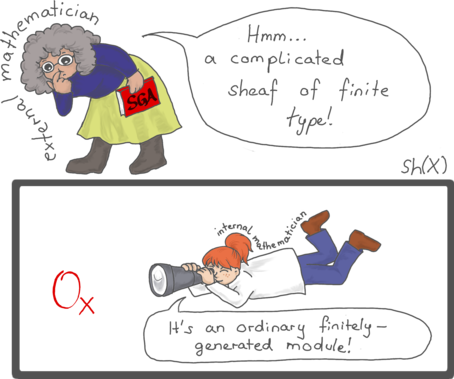
\includegraphics[width=0.5\textwidth]{external-internal-small.png}
\end{figure}
我们可以使用这种相似的对应关系大大简化一些证明.
但是仔细考察这个对应关系, 会发现排中律没有对应.
因此, 几何学家可以选择在经典逻辑中写下繁琐且难以阅读的证明,
或者选择在一种构造主义的语言中写出简洁的证明. 这种
语言是\textbf{内语言}, 我们会在 \ref{category:inner}~节
介绍. 注意这并不是说放弃了排中律. 即使我们认为排中律成立,
这也仅仅是在外部成立, 而在外部进行证明时, 我们就要处理
譬如“有限型的模层”等概念. 在内语言中, 我们只需要处理
有限生成模, 而代价是不能使用排中律. 在内语言中写下的证明,
都可以翻译成外部语言中对复杂几何对象的操作. 有代数几何
基础的读者可以参阅~\cite{blechschmidt:2021:internal}.
插图取自\href{https://github.com/iblech/internal-methods}{此处},
这里也含有\cite{blechschmidt:2021:internal}的一份
副本, 以及许多相关的讲座幻灯片.

\subsection{经典逻辑的Curry--Howard对应}\label{ch:classical}

除了研究不含排中律的逻辑之外, 另一个方向自然的问题就是
经典逻辑是否有 Curry--Howard 对应. 答案是肯定的.
首先, 我们可以直接将排中律强行加入作为公理, 也就是直接
加入一个没有定义的常量 \(\cons{lem}\). 但是这样的缺陷是
只有排中律一条规则是公理, 其余的逻辑规则都是自然从类型论
中导出的. 同时其余的逻辑规则都有对应类型论中的判值相等.
而由于 \(\cons{lem}\) 未定义, 它没有对应的判值相等规则.
这使得类型论的性质受到一定的破坏.

那么有没有将排中律自然地加入到类型论中的方法呢?
将排中律(或者其等价形式)直接对应到类型, 我们得到的就是
计算机科学中\textbf{计算续体}的概念.

在计算机语言中,
有时候需要将控制权的流向倒转, 方便组织程序.
计算续体用数学语言描述, 就是有一个“洞”的表达式,
如 \(2 \times (3 + \sin \square)\).
它表达了\emph{后继计算}的概念. 即将 \(\square\) 算出来
之后, 后继的计算是取正弦, 加\(3\) 并乘以 \(2\).
在一些计算机语言中, 提供了一个用于获取计算续体的功能,
称作 \(\cons{call/cc}\). 考虑表达式
\[2 \times [3 + \sin(\cons{call/cc}(f))],\]
其中 \(f\) 是某个函数.
此时计算机会将\(\cons{call/cc}\)的计算续体, 也就是
\(u = 2 \times (3 + \sin \square)\) 提取出来.
紧接着, 计算机会求值 \(f(u)\).
如果 \(f\) 的程序中使用了 \(u\), 即给
\(u\) 这个计算续体提供了一个数值 \(x\),
那么程序就会开始计算 \(u[x]\), 也就是
\(2 \times (3 + \sin x)\). 我们设整个程序最终的
类型是 \(\beta\), 计算续体的洞的类型是 \(\alpha\),
那么计算续体本身的类型就应该是 \(\alpha \to \beta\),
因为给它提供一个 \(x : \alpha\), 它就会继续计算得出
一个 \(\beta\) 类型的值. \(f\) 需要接收一个计算续体,
计算出 \(\alpha\) 类型的值, 因此
\(f : (\alpha \to \beta) \to\alpha\). 最后,
\(\cons{call/cc}\) 接收 \(f\), 输出一个 \(\alpha\)
类型的值, 因此
\[\cons{call/cc} : ((\alpha \to \beta)\to\alpha)\to\alpha.\]
细心的读者可以发现, 这就是前文讲述的Peirce定律! 由于
Peirce定律与排中律等价, 我们就可以得到排中律的
Curry--Howard 对应.

还有另一个直接得到排中律的对应方法. 我们需要
\(\cons{lem} : \alpha + (\alpha \to \mathbf 0)\),
回忆 \(\mathbf 0\) 是空类型, 对应假命题.
对此, 程序直接给出第二种可能, 即 \(\alpha \to \mathbf 0\).
如果接下来我们始终没有利用这个函数, 则
这个函数是什么都不影响结果. 假如在某个时刻我们利用了
这个函数, 那么这必然是因为我们提供了一个元素 \(x : \alpha\)
作为参数. 此时, 程序跳转到一开始, 并且“反悔”,
给出第一种可能. 因为此时程序已经得到了一个元素 \(x : \alpha\),
因此它只需要直接给出这个元素即可.

注意到, 尽管这确实给出了一种类型论的解释, 但是它引入了“反悔”的可能,
或者说引入了\emph{不确定性}. 因此这就破坏了一些好的性质.
我们还有一些其他的引入经典逻辑的方式, 如 \(\lambda\mu\)-演算,
极化逻辑等等. 它们都是对好性质的权衡: 每一种都会保留
一些类型论的好性质, 而破坏另一些性质.

\chapter{Martin-L\"of类型论}\label{martinlof}

Martin-L\"of 在 70 年代前后提出了多个类似的类型论.
其中最本质的特征在于接下来介绍的相等类型. 因此我们会把
具有类似特征的其他类型论也归到此类介绍.

我们首先回顾一下之前遇到的类型. 我们有依值函数的
\(\Pi\)-类型, 还有 \(\Sigma\)-类型表示后者的类型依赖于
前者的值有序对的类型. 一般的函数类型 \(\to\) 与乘积类型
\(\times\) 可以分别表示为它们的特殊情况.
在纯类型系统中, 我们介绍了类型的
类型 (如 \(\cons{type}, \cons{kind}\) 等) 对类型系统
的影响. 接下来我们会称这些对象为\textbf{宇宙}.

我们可以继续引入类型, 例如自然数. 首先有两种构造自然数
的方式:一种是 \(\cons{zero} : \mathbb N\); 一种
是给定一个自然数 \(n : \mathbb N\), 取它的后继
\(\cons{succ}(n) : \mathbb N\). 我们称
\(\cons{zero}\) 与 \(\cons{succ}\) 为\textbf{构造子}.
除了能够构造自然数之外, 我们还需要能够使用
自然数.\footnote{构造子就是\emph{输出}是自然数的函数
(\(\cons{zero}\)是有零个参数的函数), 而我们需要\emph{输入}是自然数的函数.
在数学中我们经常遇到的\emph{泛性质}就是类似的思想.}
Curry--Howard对应在这里又发挥了神奇的作用:用于证明命题的
归纳法与用于定义函数的递归定义法, 实际上是同一件事情!
考虑\textbf{消去子}
\[\cons{elim} :
\prod_{P : \mathbb N \to \cons{type}}
P(\cons{zero}) \to
\left[\prod_{m : \mathbb N} P(m) \to P(\cons{succ}(m))\right]
\to \prod_{n : \mathbb N} P(n).\]
回忆之前提到的使用嵌套的函数类型表示多个参数的函数的技巧.
同时这里 \(\Pi\)-类型的优先级最低. 如果从逻辑的视角阅读
这个类型, 我们得到的就是
\begin{quotation}
对于所有含有变量 \(n : \mathbb N\) 的命题 \(P(n)\),
如果 \(P(\cons{zero})\) 成立, 并且对于每个
\(m : \mathbb N\), \(P(m)\) 可以推出 \(P(\cons{succ}(m))\),
那么命题就对所有的 \(n\) 成立.
\end{quotation}
这无疑就是归纳法. 而另一方面, 如果我们代入 \(P(n) = \mathbb N\),
那么这个类型就变成了
\[\underbrace{\mathbb N}_{f(0)} \to
[\underbrace{\overbrace{\mathbb N}^{m} \to \overbrace{\mathbb N}^{f(m)} \to \mathbb N}
_{\text{利用 \(m\) 与 \(f(m)\) 表达 \(f(m+1)\)}}] \to
\underbrace{\mathbb N \to \mathbb N}_{\text{得到 \(f\)}}.\]
这就是递归定义. 作为例子, 如果我们令
\(f(0) = 0\), \(f(m+1) = f(m)+2\), 那么
\(f\) 就是将输入乘以\(2\)的函数. 具体写出来就是
\[\cons{elim}\, P\,0\,\lambda m u. \cons{succ}(\cons{succ}(u))\]
这里用了类似之前的记号, \(fmn\) 表示函数 \(f\) 接受两个参数 \(m\) 与 \(n\).
读者可以自行和类型比对. 在\cite{friedman:2018:typer}中
作者用谈话的形式, 趣味十足地讲解了类似的各种构造,
读者可以参考. 对于一般的 \(P\), 这就是依赖类型下的递归.
譬如如果定义了向量空间的概念, 我们可以用消去子构造一个函数,
输入 \(n\), 输出 \(n\)维向量空间中的零向量. 这样就要求
\(P(n)\) 是 “\(n\)维向量空间” 这个类型, 因此依赖于 \(n\).

为了递归能够成立, 我们还要引入相关的等式. 我们在之前也
已经为函数类型引入了等式. 这实际上是表达式上的等价关系.
如果我们定义了一个函数 \(f = \cons{elim}\,P\,z\,s\),
那么我们希望 \(f(\cons{zero}) = z\), 并且
\(f(\cons{succ}(n)) = s\,n\,f(n)\). 我们用
阿拉伯数字简写自然数, 那么就有
\[f(3) = s\,2\,f(2) = s\,2\,(s\,1\,f(1)) = s\,2\,(s\,1\,(s\,0\,z)).\]
这些类型可以推广到一般的\textbf{归纳类型}, 以及
更强大的一些变体, 如 Martin-L\"of 引入了 W-类型的概念.
我们不详细介绍.

\section{相等类型}
数学中最常见的命题就是两个对象的相等. 因此由 Curry--Howard
对应, 我们应该有一个类型反映这一点. 对于两个同类型的元素
\(x,y : A\), 我们有\textbf{相等类型} \(x =_A y\).\footnote{这
在文献中有许多不同的记号. 有些文献使用 \(\equiv\).
还有一些文献直接使用 \(\cons{Id}_A(x,y)\).}
如果没有歧义, 可以简写成 \(x = y\).

注意这和我们之前使用的等号含义有所区别. 之前使用的等号,
其描述的相等性都是“不言自明”的. 如将一个复杂的表达式用
一个字母缩写, 此时我们认为这个缩写并不存在于类型论中,
只是为了人们实际书写方便而引入的. 还有如 \((\lambda x.x)y = y\)
的等式; 上面介绍了自然数可以用递归定义加法, 则
\(3 + 5 = 8\) 也是类似的等式. 这些等式在很多情况下
都是有机械的化简或者判定相等的方法的. 然而, 我们引入的
相等类型可以描述如 \(m + n =_{\mathbb N} n + m\) 或者 \(\zeta(2) =_{\mathbb R} \frac{\pi^2}{6}\)
这样的需要证明的定理. 这些显然没有机械的判定方法, 否则
数学家都要失业了!
我们称前者为\textbf{判值相等} (judgemental equality),
而后者(即相等类型)为\textbf{命题相等} (propositional equality).

命题相等还有一个特点, 就是我们可以用它们来构造更复杂的命题,
如 \(\neg (a^3 + b^3 =_{\mathbb N} c^3)\) 等等.
判值相等是表达式上的等价关系, 并不是一个类型, 因此不能
参与构造更复杂的命题.

为什么我们需要这样辨析相等的概念呢? 其实前一章中已经暗示
了这一点. 假如我们有一个 \(\mathbb R^{1+1}\) 类型
中的元素, 那么我需要能将它用于 \(\mathbb R^2\) 中.
这就需要类型论中有一个可以机械地判断的相等概念, 否则就无法
机械地判断某个表达式类型是否正确, 进而在Curry--Howard对应下
就意味着无法判断某个证明是否真的证明了命题. 一个类型论
不一定需要有命题相等, 但是一定有判值相等的概念. 当然这个概念
可以是平凡的, 比如只有字面相等的表达式才判值相等; 这就
产生了\textbf{弱类型论}(weak type theory).\footnote{Martin-L\"of
类型论又称作\textbf{内涵类型论}(intensional
type theory).} 在另一个极端, 我们也可以设定一条规则, 让命题相等
的概念和判值相等的概念重合:
\[\frac{M =_A N}{M = N}.\]
这就产生了\textbf{外延类型论}(extensional type theory).
这样的代价就是判值相等不再可以机械地判定, 因此在其中
写下一个命题的证明, 也没有明确的办法判断这是否是正确的
证明. 这三种类型论的联系可以参考~\cite{winterhalter:2018:ettwtt}.

不过, 我们还得先说明相等类型本身的规则是什么. 首先是
构造子
\[\cons{refl}_a : a =_A a.\]
这对应\emph{同一律}: 每个元素都等于其自身.
我们有对应的消去子
\[\cons{J} :
\prod_{P : \prod_{a,b:A} a = b \to \cons{type}}
\left[\prod_{c : A} P\,a\,a\,\cons{refl}_a\right] \to \prod_{a,b:A}\prod_{p : a=b} P\,a\,b\,p\]
这说的是“如果 \(P\) 对所有的 \(\cons{refl}\) 都成立,
那么它就对所有的 \(p : a=_A b\) 成立”.
在实用的类型论中, 通常会允许省略前面两个参数. 因此可以直接写做
\(P\,\cons{refl}_a\), 可以通过上下文推导出两个省略
的参数都是 \(a\). 同时我们为了方便也会将
\(\cons{refl}_a\) 省略为 \(\cons{refl}\).
类似地, 消去子和构造子的组合有一个等式, 这里不再给出.
读者可以参考~\cite{ufp:2013:hottbook}. 用字母J是因为
Martin-L\"of在论文~\cite{martinlof:1984:J}中的相等
类型使用了 I, 而下一个字母就是 J.

神奇的是, 用 J 原理就足够证明等式的各种性质, 比如对称性
\[\prod_{a,b:A} a = b \to b = a\]
与传递性
\[\prod_{a,b,c:A} a=b \to b=c \to a=c.\]
给定任何一个表达式 \(P(x)\), 如果有 \(a=b\),
那么 \(P(a) = P(b)\). 如果类型 \(A = B\), 那么
其间有一个双射. 这些性质的证明, 读者可以参考~\cite[\S1.12]{ufp:2013:hottbook}.

不过仍然有一些问题无法只靠J原理解决. 其中最简单的例子是
函数的\textbf{外延性}, 即如果两个函数逐点相等, 那么它们
相等.
\[\cons{funext} : \prod_{f,g : A \to B}
\left[\prod_{x : A} f(x) = g(x)\right] \to f = g.\]
这在Martin-L\"of类型论中是无法证明或者证伪的.
在\cite{boulier:2017:syntacticmodel}中有非常简单易懂的证明.
这可以看作是Martin-L\"of类型论的一个缺点, 也可以理解为一种优点.
比如将函数看作算法, 那么尽管两个函数逐点相等, 它们的算法不同,
计算需要的时间也不同. 因此函数外延性在研究算法复杂度时就的确是不成立的.
我们可以将这些命题作为额外的公理加入到理论中.

Martin-L\"of类型论中还有一个重要的缺憾是没有\textbf{商类型}.
在数学中, 商去一个等价关系是极其常见的操作, 但是在
Martin-L\"of类型论中很难加入对应的类型, 同时保证
类型论仍然具有好的性质. 注意我们可以直接将商类型作为
公理加入, 但是其他的类型均不需要公理, 这在审美上有一点
缺陷. 同时在证明类型论的性质时, 这种任意加入的公理一般
很难处理. 另外, 对于其他的类型, 我们都有对应的判值相等等式,
而公理只能影响命题相等, 因此判值相等的性质就被破坏了.
不过, 使用在 \ref{ch:bishop}~节中提到的广集的概念,
可以一定程度上规避这个问题. 这样做的缺点是每个广集上都
自带一个不同的等价关系作为“相等”, 因此需要时刻处理这些
额外的信息, 在严格书写证明的时候非常繁琐.

\section{自洽性}

%集合模型------相容性(...)


%与上面提到的典范性比较

\section{变体}

logical framework, Nuprl, stuff

对比 CIC 和 MLTT, predicativity

Lean (实际上是CoC + Inductive等)
液态张量.\cite{scholze:2020:liquid}

\chapter{范畴语义}

\section{局部Descartes闭范畴}

1984年, Seely在一篇文章~\cite{seely:1984:lccc}中
指出, 局部Descartes闭范畴可以和依值类型论中的许多
东西找到对应. \ref{beginning:ccc}~节中已经
介绍了Descartes闭范畴的概念, 而\emph{局部Descartes闭范畴}
只需要进一步的定义.
\begin{definition}
给定范畴 \(\mathcal C\) 中的对象 \(A\),
定义\textbf{俯范畴}(overcategory或slice category)
\(\mathcal C_{/A}\) 的对象为所有形如
\(B \xrightarrow{f} A\) 的态射. 两个对象
\(B \xrightarrow f A\) 与 \(C \xrightarrow g A\)
之间的态射为使得 \(g \circ h = f\) 成立的 \(h\) 的集合.
\end{definition}
这里的 “局部” 指的就是在俯范畴中的构造. 可以在
集合范畴的俯范畴中获取一些直觉: 每个箭头
\(f : B \to A\) 实际上把 \(B\) 拆分成了许多子集
\(B_x = f^{-1}\{x\}\). 而俯范畴 \(\textsf{Set}_{/A}\)
中的所有构造实际上都是这些子集上逐点的构造. 比如
\(B \to A\) 与 \(C \to A\) 在俯范畴中的乘积
\(D \to A\), 满足 \(D_x = B_x \times C_x\).
因此这也称为\textbf{纤维积}, 因为这恰好是每个 \(x\)
的原像 (即 \(x\) 上的\emph{纤维}) 乘起来. 在原范畴
中, 这就是拉回.
\begin{definition}
如果某个范畴的所有俯范畴都Descartes闭, 则称这个
范畴\textbf{局部Descartes闭}.
\end{definition}
特别地, 这个范畴需要有所有的拉回. 如果这个范畴含有终对象
\(1\), 那么 \(\mathcal C_{/1} \cong \mathcal C\),
从而其本身是 Descartes 闭的.

如果 \(f\) 是局部 Descartes 闭范畴 \(\mathcal C\)
中的对象, 那么我们立即有一个函子
\[f_! : \mathcal C_{/B} \to \mathcal C_{/A}\]
描述了箭头的复合. 而由于存在所有的拉回, 有另外一个函子
\[f^* : \mathcal C_{/A} \to \mathcal C_{/B}\]
把每个箭头 (即 \(\mathcal C_{/A}\) 中的对象) 与
\(f\) 取拉回. 进一步由于存在局部的函数对象, 可以构造
第三个函子
\[f_* : \mathcal C_{/B} \to \mathcal C_{/A}.\]
事实上, 这三个函子构成伴随链\(f_!\dashv f^*\dashv f_*\).
读者可以阅读本人的一篇文章~\cite{me:2022:lccc}, 是对局部
Descartes闭范畴, 以及其对应的伴随函子 \(f_!\dashv
f^*\dashv f_*\) 的一份比较友好的介绍. 事实上, 这三个
函子可以给出局部Descartes闭范畴的等价定义.
\begin{theorem}
任给一个范畴, 则其中所有的态射 \(f\) 都一定有对应的
\(f_!\) 函子. 这个范畴是Descartes完备的, 等价于
每个 \(f_!\) 函子都存在连续的两个伴随函子
\[f_!\dashv f^*\dashv f_*.\]
\end{theorem}

Seely 在 \cite{seely:1984:lccc} 中的重要观察是,
这三个函子对应了依值类型论中重要的三个操作:
\(\Sigma\)-类型, 代入, \(\Pi\)-类型.

我们将每个箭头 \(p : E \to B\) 看作是一族依值类型:
\[x:B \vdash E(x)\,\mathrm{type}\]
这里, 每个 \(E(x)\) 的大致含义就是
原像 \(p^{-1}\{x\}\). 当然, 这只是集合范畴给出的直觉,
一般范畴里不一定有“原像”的概念. 此时如果有一个元素
\(e : 1 \to B\), 那么我们构造拉回
\[\begin{tikzcd}
  {E'} & 1 \\
  E & B
  \arrow[dashed, from=1-1, to=1-2]
  \arrow[from=1-1, to=2-1]
  \arrow["p", from=2-1, to=2-2]
  \arrow["e", from=1-2, to=2-2]
  \arrow["\lrcorner"{anchor=center, pos=0.125}, draw=none, from=1-1, to=2-2]
\end{tikzcd}\]
则此时 \(E'\) 如果在集合的范畴中考虑, 就是
\(p^{-1}\{e\}\). 换句话说, \(e^{*}\) 函子把
\(p : E \to B\) 射到 \(E' \to 1\), 对应类型论中的
\[\vdash E(e) \, \text{type}\]
而对于一般的情况, \(e\) 本身也可能有变量, 即
\(e : A \to B\). 那么这时候得到的就是
\[a : A \vdash E(e(a)) \, \text{type}\]
由此可以看出, 拉回 \(e^*\) 对应的类型论操作
是\emph{代入}. 进一步, 如果有这个箭头 \(p : E \to B\)
表示一族类型 \(x:B \vdash E(x)\),
那么它与 \(\iota : B \to 1\) 进行复合, 得到的
就是全空间 \(E\), 换句话说就是 \(\Sigma\)-类型:
\[\vdash \sum_{x:B}E(x) \, \text{type}\]
因此可见 \(\iota_!\) 函子对应的是取 \(\Sigma\)-类型
的操作. 同样, 如果将 \(1\) 改成一般的对象\(A\), 即有
\(a : A \vdash B(a)\) 类型, 此时有
\[a : A \vdash \sum_{x : B(a)} E(x)\, \text{type}\]
最后, \(\iota_*\) 对应 \(\Pi\)-类型, 与 \(\Sigma\)-类型
是对偶的, 留给读者作为练习.

当然, 这只覆盖了三个构造. 细心的读者可能也有其他的疑惑:
为什么一些箭头被看成依值类型, 而另一些箭头 (比如 \(e\))
被看成元素? 类型论里其他的构造, 比如自然数类型, 宇宙类型
等, 需要如何翻译? 这些问题促使数学家发展了更加细化的
理论. 如今我们有一系列的定义, 各自有细微的差别, 并且
各有优劣. 它们就是依值类型论的\textbf{模型}.

\section{意象}
意象有几何学与逻辑学两方面的起源~\cite{mclarty:1990:toposhistory}.
一方面是1960年代, 几何学家Grothendieck在代数几何的研究中
由\emph{层}(sheaf)的概念提出了Grothendieck意象的定义.
另一方面, 逻辑学家Lawvere在试图用范畴重新刻画集合时
提出了“集合范畴的初等理论”, 缩写为ETCS; 他接下来
受到提出论域论的Dana Scott与Grothendieck的启发, 在70年代初
与Tierney一起给出了意象的公理化定义. 意象 --- 或者为了强调
区别, 称为\emph{初等意象} --- 比 Grothendieck 意象
更加一般. 因此, 我们从几何的角度入手, 介绍意象的概念.
这部分内容参考了~\cite{joyal:2019:topologie}.

\subsection{拓扑空间与位象}
首先, 我们回顾拓扑空间的定义.
\begin{definition}
一个集合 \(X\) 上的\textbf{拓扑}是一族子集 \(\Omega \subseteq \mathcal P(X)\),
使得 \(\varnothing, X \in \Omega\), 并且
\(\Omega\) 在有限交和无限并下封闭. 配备了拓扑的集合称为%
\textbf{拓扑空间}. \(\Omega\) 中的集合称为\textbf{开集}.
\end{definition}
然而, 这个定义并非浑然天成: 我们极少会考虑不满足 T\(_0\)
分离公理的空间.
\begin{definition}
如果某个拓扑空间 \(X\) 中任意两个不同的点都有一个开集
包含其中恰好一个点, 则称这个拓扑空间为 T\(_0\) 的,
或称之为 \textbf{Kolmogorov 空间}.
\end{definition}
对于任何一个拓扑空间, “所有开集要么同时包含, 要么同时不包含两个点\(x,y\)”
构成一个等价关系. 我们可以商去这个关系得到一个 T\(_0\) 拓扑空间.
这说明拓扑空间的定义虽然简洁, 但是点和开集的关系并不是
严丝合缝, 而是有一些松动; 我们使用这个定义仅仅是因为
这些瑕疵不影响大局. 或许我们可以先不考虑点集, 仅仅看开集
上的关系. 这引出了\textbf{无点拓扑学}的研究.

首先, 在序理论中有格(lattice)的概念, 即某个偏序, 满足
任意两个元素有下确界和上确界, 称为交(meet)和并(join).
如果可以取任意的并, 则称其为\textbf{并-半完备格},
因为任意一族元素都有上确界, 但下确界则不然.
最后, 如果交和并之间有分配律:
\[x \wedge \bigvee_{\alpha \in I} y_\alpha
= \bigvee_{\alpha \in I} (x \wedge y_\alpha),\]
则称其为\textbf{并-半完备分配格} (frame).

对于任何一个拓扑 \(\Omega\), 以集合的包含
关系作为偏序, 则交与并就是集合的交与并. 那么拓扑的定义
保证了 \(\Omega\) 形成一个并-半完备分配格. 因此我们
可以看到, 并-半完备分配格绕过了点集, 直接刻画了开集
的概念. 我们把拓扑空间 \(X\) 的开集构成的格记作 \(\Omega(X)\).

这里需要注意的是, 并-半完备分配格中实际上也一定有任意
的下确界. 这是因为对于任何一族元素 \(A\), 考虑集合
\(\{x \mid \forall y \in A, x \le y\}\). 则这个
集合的上确界就是 \(A\) 的下确界. 因此所有的并-半完备格
也是交-半完备格, 从而也是完备格. 例如在开集构成的并-半
完备格中, 下确界是\emph{交集的内部}, 而不是交集 (因为
交集不一定是开集). 那么为什么需要区分这三个概念呢? 因为
我们要考虑这些代数结构之间的同态.

\begin{definition}
给定两个并-半完备分配格 \(X, Y\), 从 \(X\) 到 \(Y\)
的\textbf{同态}是一个单调函数 \(f : X \to Y\), 满足
\[f(x\wedge y) = f(x) \wedge f(y),\]
\[f\left(\bigvee_{\alpha \in I} x_\alpha\right)
= \bigvee_{\alpha \in I} f(x_\alpha).\]
\end{definition}

而给定了交-半完备分配格, 同态则需要保持无限交. 因此这三个
概念的同态定义不同. 正如Marx所说:“人是一切社会关系的总和.” 社
会关系改变, 就会极大地改变人的属性. 在这里, 尽管这三种
数学对象孤立来看是完全相同的, 但是它们的同态定义不同却
导致了完全不同的性质.

回到拓扑空间上来, 拓扑空间的连续映射是否对应了并-半完备
分配格之间的同态呢? 答案或许有些出乎意料.
\begin{theorem}
给定拓扑空间 \(X, Y\), 则\(X \to Y\)的连续映射
对应一个反向的同态 \(\Omega(Y) \to \Omega(X)\).
\end{theorem}
当然, 从定义看这是显然的, 连续性的定义要求开集
的\emph{原像}是开集, 因此这里箭头的反向并不奇怪.

并-半完备分配格是一种代数结构. 它的态射对应着拓扑空间
的\emph{反向}连续映射. 因此, 如果我们希望将并-半完备分配
格看成几何结构时, 我们称之为\textbf{位象} (locale).
换句话说,一个位象就是一个并-半完备分配格, 但是位象之间
的\textbf{连续映射}是反向的同态. 同态
方向的改变虽然仅仅是语言上的轻微改变, 但是这对
思考方式会有重要的影响.\footnote{Marshall Stone 是
最早发现这样的对偶的人: 每个Boole代数都可以实现为一族包含空集和全集,
在有限交、有限并、补集操作下封闭的集合 (在实分析中称
为\textbf{集合域}). 这也可以等价表述为一个紧致完全
不连通Hausdorff拓扑空间, 现在我们称作\textbf{Stone}空间.
Boole代数的同态和Stone空间之间反向的连续映射有一一对应.}

位象的余积(即空间的不交并)对应着并-半完备分配格的积.
这在拓扑空间上来看很明显: 两个拓扑空间的不交并上的开集,
与两个空间各自选择一个开集构成的有序对一一对应.
而位象的积(即空间的Descartes积)对应这个并-半完备分配格
的余积. 而一般代数结构的余积都比较复杂, 例如群的余积就
是\emph{自由积} \(G * H\). 这里也是类似的, 我们不详细
描述其构造. 从这些简单的例子就可以看出代数与几何之对偶的
优美.

对于位象的研究, 还有一个呼之欲出的问题: 位象与拓扑空间
之间的关系如何? 换句话说, 在这两者之间转换会不会损失某些
信息? 用范畴论的语言可以更精确地描述. 给定拓扑空间与
连续映射构成的范畴 \(\mathsf{Top}\), 和位象与连续映射
构成的范畴 \(\mathsf{Loc}\), 我们希望研究这两者之间
的关系.

由刚才的介绍, 我们知道 \(\mathsf{Loc}\) 将所有箭头
反转, 得到的就是并-半完备分配格构成的范畴 \(\mathsf{Frm}\).
我们也已经知道对于每个拓扑空间都可以取其开集构成的位象; 而
拓扑空间的连续映射对应位象之间的连续映射. 用范畴论的语言
来说, 我们有一个函子
\[\mathsf{Top} \xrightarrow{\Omega} \mathsf{Loc}
= \mathsf{Frm}^{\mathrm{op}}.\]
如果某个拓扑空间不满足 T\(_0\) 公理, 那么从拓扑的角度
存在两个点是完全无法分辨的. 因此我们会损失关于这两个点
的区别的信息, 换言之, \(\Omega\) 函子不是范畴等价.
不过, 这里仍然可以看看最多可以得到什么.
我们希望构造一个反向的函子 \(\mathrm{Pt} :
\mathsf{Loc} \to \mathsf{Top}\), 使得它尽可能地
是 \(\Omega\) 的逆. 为此, 我们需要尽可能地还原出拓扑
空间里的点 (这也是这个函子名字的来源).

我们可以使用范畴论风格的语言来重新表述“点”的概念: 拓扑空间
\(X\) 中的点无非就是单点拓扑空间 \(1 \to X\) 的连续
映射组成的集合. 这里 \(1\) 在范畴论中扮演的角色就是
终对象. 因此同样地, 我们在 \(\mathsf{Loc}\) 范畴中考虑
\(1 \to X\) 的态射, 也就是在 \(\mathsf{Frm}\) 范畴中
\(X \to 0\) 的态射.

\(\mathsf{Frm}\) 中的始对象 \(0\) 有两个元素, 一个
大于另一个, 不妨写作 \(\top \ge \bot\). 这对应拓扑
空间 \(1\) 的开集, 恰好有全集与空集两个.
\(X \to 0\) 的态射则需要给每个元素赋予 \(\top, \bot\)
之一, 并且需要单调, 并且保持有限交与无限并. 直观上,
赋予 \(\top\) 表示开集包含这个点, 而 \(\bot\) 表示
开集不包含这个点. 一个态射 \(X \to 0\) 通过给每个开集
赋予 \(\top,\bot\) 来试图描述拓扑空间中的某个点. 读者
可以试图验证在 Hausdorff 拓扑空间上, 这的确恰好可以
复原其点集. 这说明我们走在正确的方向上了.

不过, Hausdorff 性仅仅是充分条件. 我们可以给出一个
充分必要条件:
\begin{definition}
一个拓扑空间是\textbf{朴实}(sober)的, 当且仅当对于
任何无法被非平凡地表示为两个闭集的并的非空闭集 \(K\),
都存在唯一一个点, 使得 \(K\) 是这个点的闭包.
\end{definition}
读者可以进一步在无点拓扑学的课本中了解这个条件与其他分离
条件之间的关系. 特别地, 它强于 T\(_0\) (Kolmogorov),
但弱于 T\(_2\) (Hausdorff).

有了点集之后, 这个点集上的拓扑就可以继续如上文所说的方式
恢复出来. 这样我们就得到了一个函子 \(\mathrm{Pt} :
\mathsf{Loc} \to \mathsf{Top}\). 我们刚才看到了
拓扑空间能被恢复的条件. 那么反过来, 给定一个位象生成的
对应的拓扑空间, 是否还能恢复原来的位象呢? 这同样给出一个
条件
\begin{definition}
一个位象\textbf{有足够的点}\footnote{英文为 have enough
points, 或者称为 spatial.}当且仅当对于任何两个元素
\(u, v\), 存在某个点 (即对应的并-半完备分配格的态射
\(X \to 0\)) 对于这两个元素的赋值不同.
\end{definition}
范畴论的一个重要观察就是, 如果两个范畴“几乎”等价,
那么你往往可以期待它们之间有一对伴随函子. 这里也不例外.
拓扑空间与位象之间的关系可以被总结为下面的定理:
\begin{theorem}
有一对伴随函子
\[\begin{tikzcd}
{\mathsf{Top}} && {\mathsf{Loc}}
\arrow[""{name=0, anchor=center, inner sep=0}, "\Omega", shift left=1, curve={height=-6pt}, from=1-1, to=1-3]
\arrow[""{name=1, anchor=center, inner sep=0}, "{\mathrm{Pt}}", shift left=1, curve={height=-6pt}, from=1-3, to=1-1]
\arrow["\dashv"{anchor=center, rotate=-90}, draw=none, from=0, to=1]
\end{tikzcd}\]
两侧的像分别是朴实拓扑空间与有足够的点的位象. 同时,
两个函子限制在这两个完全子范畴上是范畴的等价.
\end{theorem}

\subsection{层与意象}
有了这样把拓扑空间中的点放在次要地位, 而将开集作为更根本的
数学对象的思想, 我们可以进一步引出意象的概念了.
Grothendieck提出层的概念, 是为了更好地整理代数几何中
复杂的数学对象. 层可以看作是一类数学对象的刻画:
\begin{itemize}
\item 某个拓扑空间中, 定义在开集上的连续函数;
\item 微分流形中, 定义在开集上的可微函数;
\item 代数几何中, 某个环的素谱(spectrum)上的正则函数.~\cite[第二章, 例1.0.1]{hartshorne:1977:ag}
\end{itemize}
它们的一些重要特征:
\begin{itemize}
\item 大开集上的连续函数可以限制到小开集上, 仍然是连续函数;
\item 几个小开集上的连续函数, 如果在交集上相等, 那么就可以粘合成并集上的连续函数.
\end{itemize}
因此我们可以提炼出一个定义.
\begin{definition}
给定拓扑空间 \(X\), 一个\textbf{层} \(\mathscr F\) 是一组数据:
\begin{itemize}
\item 对每个开集 \(U \subseteq X\) 取定一个集合,
记作 \(\mathscr F(U)\) 或 \(\Gamma(U, F)\).
称作 \(\mathscr F\) 在 \(U\) 上的\textbf{截面}.
\item 对于开集的子集 \(U \subseteq V\), 有函数
\(\mathrm{res}_{V,U} : \mathscr F(V) \to \mathscr F(U)\),
称为截面的限制.
\end{itemize}
它们满足一些性质:
\begin{itemize}
\item \(\mathrm{res}_{U,U}\) 是恒等映射.
\item \(\mathrm{res}_{V, W}\circ \mathrm{res}_{U,V} = \mathrm{res}_{U, W}\).
\item 给定开覆盖 \(U = \bigcup_{i\in I} U_i\),
对于任何一组 \(f_i \in \mathscr F(U_i)\), 满足
\[\mathrm{res}_{U_i, U_i \cap U_j}(f_i)
= \mathrm{res}_{U_j, U_i \cap U_j}(f_j),\]
则存在唯一的 \(f \in \mathscr F(U)\), 使得
其限制在各个 \(U_i\) 上等于 \(f_i\). 这条公理称作
粘合公理. 去掉这条公理, 则这是\textbf{预层}的定义.
\end{itemize}
\end{definition}
称 \(\mathscr F(U)\) 为截面, 继承自纤维丛的截面
的概念. 因为每个纤维丛上的截面的确构成层. 对于两个层,
我们自然可以写出它们之间的态射:
\begin{definition}
给定两个层 \(\mathscr F, \mathscr G\), 它们
之间的态射是一组映射 \(\varphi_U : \mathscr F(U) \to \mathscr G(U)\),
使得下图交换:
\[\begin{tikzcd}
{\mathscr F(U)} & {\mathscr F(V)} \\
{\mathscr G(U)} & {\mathscr G(V)}
\arrow["{\mathrm{res}_{U,V}}", from=1-1, to=1-2]
\arrow["{\mathrm{res}_{U,V}}"', from=2-1, to=2-2]
\arrow["{\varphi_U}"{description}, from=1-1, to=2-1]
\arrow["{\varphi_V}"{description}, from=1-2, to=2-2]
\end{tikzcd}\]
\end{definition}
由此, 对于任何拓扑空间 \(X\), 我们都定义了其上
的\textbf{层范畴} \(\mathsf{Sh}(X)\).
读者可以轻松地把这些定义全部类比到位象上去.
可以证明 \(\mathscr F(\varnothing)\) 必须为单点集.
因此, 在单点拓扑空间上的层, 完全由全集上的截面决定.
因此单点拓扑空间上的层范畴等价于集合范畴 \(\mathsf{Set}\).

这些定义到1950年代已经成为主流数学的重要工具. 然而, 在
代数几何中, \(X\) 上只有拓扑信息是完全不够的. 例如在
一维情况下, Zariski 拓扑就是余有限拓扑, 因此 Zariski
连续的函数 \(\mathbb A^1 \to \mathbb A^1\)
只需要保证每个点的原像有限 (或者是常函数), 但是我们只关心有理函数!
Grothendieck 为此推广了层范畴的定义, 以便包含这些
信息.

注意到, 我们并不需要用到 \(X\) 这个拓扑空间的全部信息.
因此正如位象的定义一样, 我们绕过拓扑空间本身, 直接找到需要的信息进行定义.
对于预层的定义, 我们只需要知道开集上的包含关系, 也就是
任何一个偏序. Grothendieck 将这里的偏序推广成了
范畴. 可以看出, 给定某个范畴 \(\mathcal C\), 一
个\textbf{预层}就是函子 \(\mathcal C^{\mathrm{op}}
\to \mathsf{Set}\). 而对于粘合公理, 我们只需要
知道开集的交集与“开覆盖”的概念.

注意到两个子集 \(X_1, X_2 \subseteq X\) 的交
集\footnote{交集只有对某个共同集合的子集谈论才有意义,
任意两个集合的交集只有研究物料集合
论(material set theory)时才会
遇到, 在一般数学中没有任何应用.}可以
用范畴论的语言表示为拉回
\[\begin{tikzcd}
{X_1 \cap X_2} && {X_2} \\
\\
{X_1} && X
\arrow[hook, from=3-1, to=3-3]
\arrow[hook, from=1-3, to=3-3]
\arrow[from=1-1, to=3-1]
\arrow[from=1-1, to=1-3]
\arrow["\lrcorner"{anchor=center, pos=0.125}, draw=none, from=1-1, to=3-3]
\end{tikzcd}\]
因此我们只需要再定义什么是开覆盖就可以了. 换句话说,
对于每一组箭头 \(\{f_i : U_i \to U\}\), 我们需要
决定它是否覆盖了 \(U\). 当然, 并不是所有的选择都能得到
好的性质. 因此Grothendieck提出了一组要求, 满足这些
要求的则被称作\textbf{Grothendieck拓扑}.\footnote{现在
使用的Grothendieck拓扑的定义比这个定义略微更一般一些,
因为有时候范畴中没有所需要的拉回. 读者可以参
阅\cite{johnstone:2008:elephant}中的讨论.}
\begin{itemize}
\item 每个同构本身构成覆盖.
\item 如果 \(\{f_i : U_i \to U\}\) 覆盖了 \(U\),
并且 \(\{g_{i,j} : V_{i,j} \to U_i\}\) 覆盖了 \(U_i\), 那么
\(\{f_i \circ g_{i,j} : V_{i,j} \to U\}\) 也覆盖了 \(U\).
\item 如果 \(\{f_i : U_i \to U\}\) 覆盖了 \(U\),
并且有态射 \(V \to U\) (类比拓扑空间中的子集 \(V \subseteq U\)),
那么拉回 \(U_i \times_U V\) (我们上面提到这类比拓扑空间中的交集)
均存在, 并且拉回得到的一组态射
\(U_i \times_U V \to V\) 也构成覆盖.
\end{itemize}
配备了Grothendieck拓扑 \(J\) 的范畴 \(\mathcal C\)
被称为\textbf{景}(site). 注意每个拓扑空间上的开集
都自动构成景. 可以在景上叙述粘合公理的推广.
\begin{definition}
考虑 \(\mathcal C\) 上的预层 \(\mathscr F\).
对于任何一组覆盖 \(\{f_i : U_i \to U\}\), 都有
一个交换方 (不一定是拉回):
\[\begin{tikzcd}
{\mathscr F(U_i \times_U U_j)} && {\mathscr F(U_j)} \\
\\
{\mathscr F(U_i)} && {\mathscr F(U)}
\arrow["{\mathscr F(f_i)}", from=3-3, to=3-1]
\arrow["{\mathscr F(f_j)}"', from=3-3, to=1-3]
\arrow[from=3-1, to=1-1]
\arrow[from=1-3, to=1-1]
\end{tikzcd}\]
注意箭头的方向. 如果对于一组元素 \(x_i \in \mathscr F(U_i)\),
每对 \(x_i, x_j\) 映射到 \(\mathscr F(U_i \times_U U_j)\)
上相等, 那么存在唯一的 \(x \in \mathscr F(U)\) 使得
\(x_i\) 是 \(x\) 在 \(\mathscr F(f_j)\) 下的像.
满足上述条件的预层称为\textbf{层}.
\end{definition}
可以用更加精炼的范畴语言重新叙述. 上面的交换方的左侧
和上方的态射分别可以合并得到态射
\[\coprod_{i \in I} \mathscr F(U_i)
\rightrightarrows \coprod_{i,j \in I} \mathscr F(U_i \times_U U_j).\]
粘合公理则是说这两个态射有等值子
\[\mathscr F(U) \to \coprod_{i \in I} \mathscr F(U_i)
\rightrightarrows \coprod_{i,j \in I} \mathscr F(U_i \times_U U_j).\]

有了这个定义, 我们就可以定义例如 Zariski 景、
平展景、Nisnevich景等等概念, 将复几何中的技术应用到
代数几何上来.
对于更多有关的几何讨论, 读者可以参阅~\cite{maclane:2012:sheaves}.
而意象论最重要的书籍则是~\cite{johnstone:2008:elephant},
因其书名被戏称为“大象书”.

我们现在可以给出意象的一种定义:
\begin{definition}
一个\textbf{Grothendieck意象}是某个景上所有的层构成的范畴.
\end{definition}
当然, 意象的内涵比这要丰富很多. Giraud给出了某个范畴
是Grothendieck意象的一组充分必要条件, 因此在不涉及几何
的材料中也经常把这组条件直接作为Grothendieck意象的定义.
另外, 也有许多书中首先定义我们后面会介绍的初等意象, 然后
将Grothendieck意象定义为满足某些条件的初等意象. 从某种
意义上来说, 意象这个概念正如一头大象. 每种定义都如盲人
摸象一般, 表面上看似乎分别给出了截然不同的数学概念, 但
实际上都表现了意象的一个方面.

意象的定义是一类范畴, 因此它们之间态射最明显的定义
是满足某些条件的函子. 但是意象作为一类几何对象, 它们之间
也应当有与位象类似的“反向”的态射关系. 如果它们作为代数结
构, 态射是(满足某些条件的)函子时,
Joyal~\cite{joyal:2019:topologie}称它们为logos
(试译为\textbf{道理}); 而它们构成的范畴 \(\mathsf{Logos}\)
将箭头反向就得到几何对象构成的范畴 \(\mathsf{Topos}\).
读者也可以参阅\cite{sterling:2021:thesis}的第二章.
这样, 位象就可以整合到我们的定义中:
\[\begin{tikzcd}
&& {\mathsf{Topos}} && {\mathsf{Logos}} \\
{\mathsf{Top}} && {\mathsf{Loc}} && {\mathsf{Frm}}
\arrow["\Omega", curve={height=-6pt}, from=2-1, to=2-3]
\arrow["{\mathrm{Pt}}", curve={height=-6pt}, from=2-3, to=2-1]
\arrow["{\mathsf{Sh}}", hook', from=2-3, to=1-3]
\arrow[hook', from=2-5, to=1-5]
\arrow["{(\mathrm{op})}"{description}, Rightarrow, no head, from=2-3, to=2-5]
\arrow["{(\mathrm{op})}"{description}, Rightarrow, no head, from=1-3, to=1-5]
\end{tikzcd}\]

\subsection{初等意象}

\section{内语言}\label{category:inner}

排中律

Kripke--Joyal, 推广之前的 Kripke

\chapter{同伦类型论}
\section{K原理的独立性}
我们刚才已经看到相等类型的归纳子, 也就是 J 原理. 它直觉上大致说的是
“每个 \(a = b\) 类型都只有 \(\cons{refl}\) 一个
构造器”. 但是想要表达这个直觉, 还有一个看起来很自然的写法:
\[\prod_{a,b : A} \prod_{p,q : a = b} p = q,\]
或者写成
\[\prod_{a : A} \prod_{p : a = a} p = \cons{refl},\]
注意这里不能写 \(p : a = b\), 因为这样它与
\(\cons{refl}\) 的类型不同, 就不能表达相等了.
当然, 也可以用上面的 \(\Sigma\)-类型补救一下, 写成
\[\prod_{a,b : A} \prod_{p: a = b} (a,b,p) =_{\sum_{a,b : A}a = b} (a,a,\cons{refl}).\]
上面的三个命题都是等价的. 我们将它们统称为
\textbf{K 原理}\footnote{这个名字是因为
其提出者Thomas Streicher顺承J原理的名字, 使用了下一个字母K.~\cite{streicher:1993:K}}.
令人惊讶的是, 很长一段时间中并没有人能从 J 原理推
出 K 原理. 在第\ref{martinlof}章介绍的集合模型中,
K 原理显然是成立的, 因此加入 K 公理后类型论仍然无矛盾.
进而无法证伪 K 原理. 那么反过来, 是否能证明 K 呢?

在 Martin-L\"of 类型论提出之后, K原理是否能
从 J 原理中推出, 是一个重大的未解问题.
这个问题直到1998年才被 Hofmann 等人解决~\cite{hofmann:1998:groupoid}.
而这一解决方案, 对认识类型论的内禀结构提供了重要的
方向 ------ 类型可以是群胚!

\begin{definition}
\textbf{群胚}包含以下结构:
给定一个集合 \(C\), 对于每对元素 \(x,y\in C\)
都取一个集合 \(\hom(x,y)\), 并且有乘法运算
\(a * b\) 为二元函数 \(\hom(y,z) \times \hom(x,y) \to \hom(x,z)\).
每个元素 \(x \in C\) 都有对应的单位元
\(\cons{id}_x \in \hom(x,x)\), 乘法运算满足单位律与结合律.
每个元素 \(a \in \hom(x,y)\) 都有逆元
\(a^{-1} \in \hom(y,x)\).
\end{definition}
读者可以很快验证, 每个群都是使得 \(C = \{\star\}\)
为一元集的群胚. 而另一个极端的例子, 对于任何集合 \(C\),
直接令 \(\hom(x,x) = \{\cons{id}_x\}\) 为一元集, 其它 \(\hom(x,y)\)
均为空集. 这则被称为\textbf{离散群胚}.

还有一族更加有启发性的例子:
\begin{theorem}
任给一个拓扑空间 \(X\), 令其点集为
\(C\), \(\hom(x,y)\) 为从点 \(x\) 到点
\(y\) 的道路的集合, 商去同伦关系,
乘法运算为道路拼接操作, 那么它构成一个群胚.
\end{theorem}
容易看出这是基本群的推广. 因此我们可以将群胚看成是“允许取
多个基点的群”. 我们回过头来看类型论,
用 J 原理可以很容易证明, 每个类型上都自带一个群胚结构.
我们有 \(\cons{refl} : x = x\) 为单位元,
对称性
\[\prod_{x, y : A} x = y \to y = x\]
与传递性
\[\prod_{x,y,z : A} x = y \to y = z \to x = z\]
之前也已经提到过.

因为这些全都只需要 J 原理, 因此我们可以试着构造类型论
的一个模型, 使得每个类型被解释为一个群胚. 这之中乘积
类型被解释为群胚的乘积, 等等. 最重要的是, 相等类型
\(x = y\) 被解释为集合 \(\hom(x,y)\) 上的\emph{离散}群胚.
因为当前的模型中 \(\hom(x,y)\) 只是一个集合, 没有
其他结构. 最终可以验证, 这个模型满足J原理.

构造了这个模型之后, K 原理在这个模型中的解释是什么呢?
我们可以发现它对应 “所有群胚都是离散群胚” 这个命题.
显然是不成立的. 从而我们构造了 K 原理的反模型. 上面的
讨论即证明了如下命题:
\begin{theorem}
在只有 J 原理的 Martin-L\"of 类型论中, 无法证明或者
证伪 K 原理.
\end{theorem}

% (...) pattern matching (with/without K)
\section{同伦类型论}
在上面的模型中, 每个类型都是群胚. 而由于群胚的 \(\hom\) 集合
只有集合结构, 取相等类型之后我们就得到了一个集合, 也就是
离散群胚. 但是仅仅从语法上来看, 相等类型作为群胚也有可能
是非平凡的. 换句话说, 尽管我们确定了 K 原理 (解释为“所有类型
都是离散群胚”)是不可证明的, 我们却马上有了高一层的问题, 也
就是“所有类型上的相等类型都是离散群胚”. 写成语法, 我们可以
对比一下. K原理是
\[\prod_{a,b : A} \prod_{p,q:a=b} p = q.\]
而这里说的高一层的K原理就是
\[\prod_{a,b : A} \prod_{p,q:a=b} \prod_{\alpha,\beta:p=q} \alpha = \beta.\]
很明显这可以一直继续下去. 我们不妨做个编号, K\(_{-1}\) 原理
就是
\[\prod_{a,b : A} a = b,\]
K\(_0\) 原理就是 K 原理, 而 K\(_1\) 原理就是上面说的
高一层的K原理. 以此类推有 K\(_n\) 原理.

我们已经知道用群胚模型可以得到 K\(_0\) 原理不可证明.
那么以此类推, 是否构造一个 \(\hom\) 不是集合而是群胚
的 “2-群胚”,就能得到 K\(_1\) 原理不可证明了呢? 答案是
肯定的. 这引出了 \(n\)-群胚乃至 \(\infty\)-群胚的概念.
具体的定义虽然简单但是细节繁杂, 这里不再给出. 但是相信
读者已经有了大致的图像. \(\infty\)-群胚是同伦论研究中
用到的概念. 事实上, 拓扑空间的道路就可以看
作\(\infty\)-群胚: 我们取所有的道路, \emph{不商去同伦}.
那么所有道路(也就是1-道路)并不是严格构成群胚, 因为结合律
等等式只在道路的同伦意义下成立. 换句话说结合律是道路的道路,
也就是2-道路. 而进一步, 2-道路之间也有等式. 考虑五条道路
之间的2-道路:
\[\begin{tikzcd}
& {(p\cdot q)\cdot (r\cdot s)} \\
{((p\cdot q)\cdot r)\cdot s} && {p\cdot (q\cdot (r\cdot s))} \\
{(p\cdot (q\cdot r))\cdot s} && {p\cdot ((q\cdot r)\cdot s)}
\arrow[no head, from=2-1, to=1-2]
\arrow[no head, from=2-1, to=3-1]
\arrow[no head, from=3-1, to=3-3]
\arrow[no head, from=3-3, to=2-3]
\arrow[no head, from=2-3, to=1-2]
\end{tikzcd}\]
在拓扑空间中可以证明这五条2-道路复合形成的2-道路到平凡
的2-道路一定有一条3-道路, 以此类推到任意高的 \(n\)-道路.
对于每个 \(n\), \(n\)-道路商去 \((n+1)\)-道路的同伦,
就得到了 \(\pi_n\) 同伦群. 因此提到 \(\infty\)-群胚时,
读者可以大致理解为拓扑空间.

因此, 我们对类型的崭新理解就是“类型是空间”.
在\cite{ufp:2013:hottbook}中对此有详细的论述.
我们之前的口号“类型是命题”并不是最好的对应, 事实上
只有一部分类型应该作为命题理解.
\slogan{类型不是命题!}
具体哪些类型是命题呢? 恰好是那些满足 K\(_{-1}\) 原理的类型!
这条原理实际上非常符合我们的观念.
譬如考虑偶数集 \(\{x \in \mathbb Z \mid x \equiv 0 \pmod 2\}\).
我们不会认为\(x\)是偶数的两种不同思路的证明会给出两个
不同的偶数. 因此这两个证明作为数学对象比较的时候永远是
相等的. 换句话说, 同一个命题的任何两个证明 (如果存在的话)
一定是相等的. 因此我们可以做一个定义:
\begin{definition}
称一个类型\(A\)为\textbf{命题}, 当且仅当可以证明
\[\prod_{x,y:A} x = y.\]
\end{definition}
事实上, “\(A\)是命题”这个类型也是一个命题.

进一步, 如果满足 K\(_0\) 原理, 这个类型应该称作什么呢?
由上面群胚模型的启发, 这些应该称为\textbf{集合}: 每个
集合都可以看作一个离散群胚 (或者离散拓扑空间). 我们可以
证明自然数类型是一个集合,
K\(_0\) 原理说的就是“所有类型都是集合”. 进一步, 满足
\(K_1\) 原理的被称为群胚; 满足 K\(_n\) 的则被称为 \(n\)-群胚.

\section{泛等公理}
认识到这些性质之后, 自然有了一些将类型论用于研究同伦论的
努力. Voevodsky 在 2006 年已经提出了与泛等公理相关
的性质, 但是直到 2009 年才意识到这可以直接作为公理加入
Martin-L\"of 类型论中.

这条公理来源于 \(\infty\)-群胚模型的启发, 但是我们这里只
讲述它的形式以及推论.

首先, 我们有某个函数 \(f\) 是\textbf{等价}的定义. 读者
可以参考\cite{escardo:2018:univalence}中的定义细节.
对于每个 \(f\), \(\cons{isEquiv}(f)\) 都是命题. 将
类型视作空间时, 这个定义就代表\emph{同伦等价}. 在集合上,
同伦等价就是双射. 显然我们应当有 \(\cons{isEquiv}(\cons{id})\).
我们定义 \(X\simeq Y\) 为 \(\sum_{f : X \to Y}\cons{isEquiv}(f)\),
即两个类型之间所有的等价构成的类型.

显然有 \((X = Y) \to (X \simeq Y)\), 应用 J 原理即可.
\textbf{泛等公理}说的是, 这个函数本身是一个等价. 一个立即
的推论就是
\[(X = Y) \simeq (X \simeq Y).\]
直观上来看, 它说的是“等价的类型都相等”. 事实上它有非常多
深刻的推论.
\begin{theorem}[命题外延]
等价的命题都相等: 如果有两个命题满足
\(p \iff q\), 那么 \(p = q\).
\end{theorem}
\begin{theorem}[函数外延]
如果两个函数逐点相等, 那么两个函数相等:
\[\left[\prod_{x:A} f(x) = g(x)\right] \to f = g.\]
\end{theorem}
这解决了我们在Martin-L\"of类型论中留下的问题. 但是我们
还有更加奇妙的结论:
\begin{theorem}
如果两个群同构, 那么它们相等.\footnote{更准确的说, 两个群 \(G, H\) 之间的不同同构
与类型 \(G = H\) 中的元素一一对应; 并且类型 \(G = H\) 是集合.}
\end{theorem}
注意我们的泛等公理中完全没有提到群同构, 这是自然导出的定理!
这也非常符合我们的数学实践: \(\{1,-1,i,-i\}\) 的乘法
群与 \(\mathbb Z/4\mathbb Z\) 是完全等同, 随时可以
互相替换的. 这也使得有了泛等公理之后, 在类型论里的形式化
数学比起集合论等等更加接近我们实际使用的非形式化数学语言.
这也与数学哲学中
的\textbf{结构主义}相合.~\cite{awodey:2013:structuralism}

\section{高阶归纳类型}
我们之前已经见过了许多归纳类型, 如自然数, 二叉树等等.
而在认识到类型的\(\infty\)-群胚解释后, 自然就可以对
归纳类型做出推广. 2011年 Oberwolfach 数学研究所的
一次研讨会上, Voevodsky 等人提出了许多重要的研究问题.
高阶归纳类型的想法就是在这里首次出现的.

\begin{definition}
\textbf{圆}类型有两个构造器, \(\cons{base} : \mathbb S^1\)
与 \(\cons{loop} : \cons{base} = \cons{base}\).
\end{definition}
这个类型中, \(\cons{loop}\) 就是道路的自由生成元.
利用泛等公理, 我们可以证明它的基本群是 \(\mathbb Z\)
等等与拓扑空间类似的性质. Guillaume Brunerie~\cite{brunerie:2016:number}在类型论
中证明了 \(\pi_4(\mathbb S^3) = \mathbb Z / 2\mathbb Z\).
由此看来, 高阶归纳类型真正使得类型论
变成了可以研究同伦论的工具.
当然, 除了同伦之外, \textbf{商类型}也可以作为高阶归纳
类型的特殊情况存在. 因此我们完全解决了Martin-L\"of类型论
的诸多不便之处.

我们将这些方向的类型论的各种变体泛指为\textbf{同伦类型论}.
这个词没有严格定义, 但是一般会包含泛等公理与一定量的
高阶归纳类型.

\section{泛等数学基础}
在 Oberwolfach 会议之后, 参会者搭建了%
\href{http://homotopytypetheory.org/}{同伦类型论的网站与博客},
由此进行同伦类型论的推广.
同伦类型论理论上已经可以作为数学基础使用. 正如上面所说, 它与
通常的数学语言更加接近. 此时已经有初步的形式化努力.

2012--2013年是泛等数学基础最重要的一年. 由Princeton高等研究院发起了
“泛等数学基础特别年”, 邀请了拓扑学、计算机科学、范畴论、逻辑学
等等领域的数学家参加. 其中由 Peter Aczel 提议, 尝试使用
同伦类型论书写\emph{非形式化}的数学. 这次尝试很快获得了
初步成功, 最终写出了《同伦类型论:泛等数学基础》~\cite{ufp:2013:hottbook}这本书.
它从零出发, 整理了泛等数学基础中的结论, 从同伦类型论
的角度重新叙述了集合论与范畴论, 并且给出了
实数的定义与主要性质的证明. 一方面, 写出实数理论证明
了泛等数学基础在实操上可以有效地书写一般数学; 另一方面,
这开创了\textbf{综合同伦论}(synthetic homotopy theory)的学科. 正如Euclid的
《几何原本》中并没有将平面定义为 \(\mathbb R^2\), 而是
直接从公理出发推导结论, 综合同伦论直接由类型论的基本规则
刻画同伦关系, 而无需依赖拓扑空间 \([0,1]\) 或者CW复形等等.
书中复现了许多传统同伦论中需要花费功夫证明的结论.

阅读这本书不需要类型论基础, 并且内容是开源的. 读者可以自行
下载阅读.

\section{立方类型论}


\url{https://ncatlab.org/nlab/show/cubical type theory}

BCH 模型 2013, 2017, 不适合加 HIT

ABCFHL 2019, CCHM 2017

Normalization by Sterling

XTT, 2LTT, etc.

\chapter{展望}
目前的问题:
\begin{itemize}
\item regularity
\item HIIT
\item cubical的自动化
\item 主流数学的应用
\item 机器学习
\end{itemize}

\printbibliography[title=参考文献]
\end{document}
